\makeatletter
\def\input@path{{../}}
\makeatother
\documentclass[../main.tex]{subfiles}
\begin{document}
\renewcommand{\path}{chapter_2/}
\chapter[
CBTI
]{Alchemical Free-Energy Calculations by Multiple-replica $\lambda$-dynamics: The Conveyor Belt Thermodynamic Integration
}
\chaptermark{CBTI}
\label{ch:cbti}

\aquote{``Let us learn to dream, gentlemen, and then perhaps we
shall learn the truth.''
}
{August Kekul\'e, 1865}

\begin{abstract}
A new method is proposed to calculate alchemical free-energy differences 
based on molecular dynamics (MD) simulations, called the conveyor belt 
thermodynamic integration (CBTI) scheme.
%
As in thermodynamic integration (TI), $K$ replicas of the system are 
simulated at different values of the alchemical coupling parameter $\lambda$.
%
The number $K$ is taken to be even and the replicas are equally spaced
on a forward-turn-backward-turn path, akin to a conveyor belt (CB)
between the two physical end-states.
%
And as in $\lambda$-dynamics ($\lam$D), the $\lambda$-values associated with the 
individual systems evolve in time along the simulation.
%
However, they do so in a concerted fashion, determined by the evolution
of a single dynamical variable $\Lambda$ of period $2\pi$ controlling 
the advance of the entire CB.
%
Thus, a change of $\Lambda$ is always
associated with $K/2$ equispaced replicas moving forward and $K/2$ equispaced
replicas moving backward along $\lambda$.
%
As a result, the effective free-energy profile of the 
replica system along $\Lambda$ is periodic of period $2\pi K^{-1}$
and the magnitude of its variations decreases rapidly
upon increasing $K$, at least as $K^{-1}$ \radd{in the limit of large $K$}.
%
When \radd{a sufficient number of replicas is used}, 
these variations become small, 
which enables a complete and quasi-homogeneous coverage of the $\lambda$-range
by the replica system, without application of any biasing potential. 
If desired, a memory-based biasing potential can still be 
added to further homogenize the sampling, the preoptimization of which 
is computationally inexpensive.
%
The final free-energy profile along $\lambda$ is calculated similarly to TI,
by binning of the Hamiltonian $\lambda$-derivative as a function of $\lambda$ 
considering all replicas jointly, followed by quadrature integration. 
The associated quadrature error can be kept very low owing to 
the continuous and quasi-homogeneous $\lambda$-sampling.
%
The CBTI scheme can be viewed as a \radd{continuous/deterministic/dynamical}
%dynamical 
analog of the Hamiltonian
replica-exchange/permutation (HRE/HRP) schemes, or as a correlated 
multiple-replica analog of the \radd{$\lambda$D or} $\lambda$-local elevation umbrella 
sampling ($\lambda$-LEUS) schemes.
%
Compared to TI, it shares the advantage of the latter schemes 
in terms of enhanced orthogonal sampling, {\em i.e.} the availability of 
variable-$\lambda$ paths to circumvent conformational barriers
present at specific $\lambda$-values.
%
Compared to HRE/HRP, it permits a deterministic and continuous sampling
of the $\lambda$-range, and bypasses the need to carefully
preselect a $\lambda$-ladder \radd{and a swapping-attempt frequency}.
%
Compared to $\lambda$-LEUS, it eliminates (or drastically reduces) 
the dead time associated with the preoptimization
of a biasing potential.
%
The goal of this chapter is to provide the mathematical/physical formulation 
of the proposed CBTI scheme, along with an initial application of the method 
to the calculation of the hydration free energy of methanol.
%
\end{abstract}

\clearpage
\pagebreak

%%%%%%%%%%%%%%%%%%%%%%%%%%%%%%%%%%%%%%%%%%%%%%%%%%%%%%%%%%%%%%%%%%%%%
%% Start the main part of the manuscript here.
%%%%%%%%%%%%%%%%%%%%%%%%%%%%%%%%%%%%%%%%%%%%%%%%%%%%%%%%%%%%%%%%%%%%%
%================================================================================
\section{Introduction}
%================================================================================

%The Problem and the Solution
Newly developed advanced simulation methods are routinely tested on simple one- and two-dimensional model systems. They provide valuable insights into the theory, conceptual advantages and limitations (for examples see e.g. Refs. \cite{Huber1994, Laio2002, Christ2007, Konig2012, Koenig2020, Donnini2016, Weiss2016, Lemke2018}).
While the results of new methods are published, the implementation details may not always be available or difficult to use with different computer infrastructure.
As a result, sharing, reproducing, understanding, and comparing simulation methodologies is often cumbersome.\cite{Peng2011}
To address this issue, we have developed the Ensembler package, an easy-to-use, yet powerful platform that enables fast prototyping of new methods and comparison against existing techniques using one or two-dimensional test systems.

%Global ethical goal
Ensembler is designed following the recommendations of Stodden \textit{et al.}\cite{Stodden2016} for the enhanced reproducibility of computational methods, which includes making code publicly accessible, providing documentation, and using open licensing.\cite{Stodden2016} 
Furthermore, Ensembler uses state-of-the-art software engineering tools (i.e. git,\cite{Chacon2014} MolSSI cookie-cutter,\cite{Naden2018} and binder\cite{Binder2018}/Colab\cite{Bisong2019}) to fulfill these recommendations and enable features like continuous integration and the transparent versioning of the code. 

%-------------------------------------------------------------------------------------------------------
\subsection{Method Development}
%-------------------------------------------------------------------------------------------------------

%Why not using normal MD-Packages
The lean Python3 code\cite{Vanrossum2009} of Ensembler allows for easy prototyping of new methods and comparison against a wide range of already implemented techniques. 
In contrast, the C/C++\cite{Stroustrup1995} code of traditional high-performance molecular dynamics (MD) packages (e.g. Refs. \citenum{Berendsen1995,Lindahl2001,Vanderspoel2005,Eastman2017,Brooks2009}) is more efficient but also much more complex. 
%
%What we got
The methods currently available in Ensembler are:
\begin{itemize}
	\item \textit{Model systems}: Harmonic oscillators as well as dihedral-angle, double-well, and Lennard-Jones potential-energy functions\cite{Jones1924}
	\item \textit{Sampling algorithms}: Conjugated gradient\cite{Hestenes1952} for energy minimization, Metropolis Monte Carlo (MC),\cite{Hastings1970} leap-frog integration\cite{Vangunsteren1988} for MD, and Langevin integration\cite{Brunger1984} for stochastic dynamics (SD)
	\item \textit{Enhanced sampling techniques}: Umbrella sampling,\cite{Valleau1977} simulated tempering/temperature replica-exchange simulations,\cite{Sugita1999} local elevation/metadynamics,\cite{Huber1994, Laio2002}
	\item \textit{Free-energy methods}: Free-energy perturbation (FEP),\cite{Zwanzig1954} Bennett's acceptance ratio (BAR),\cite{Bennett1976} thermodynamic integration (TI),\cite{Kirkwood1935} enveloping distribution sampling (EDS),\cite{Christ2007, Christ2008, Christ2009} $\lambda$-EDS,\cite{Koenig2020} replica-exchange EDS (RE-EDS),\cite{Sidler2016} and conveyor-belt TI\cite{Hahn2019}
\end{itemize}

%Teaching
%-------------------------------------------------------------------------------------------------------
\subsection{Teaching}
%-------------------------------------------------------------------------------------------------------

Simple model systems can also be used for teaching MD concepts to students, as they allow to intuitively understand fundamental concepts. \cite{Pohorille2010} 
Ensembler is well suited for didactic purposes because it is not only easy to use, but supports also a range of visualizations, i.e. interactive widgets, animations, and plots, which can be embedded in Jupyter notebooks.\cite{Kluyver2016}
Example Jupyter notebooks\cite{Kluyver2016} are provided in the Ensembler GitHub repository.

%================================================================================
\section{Theory}
%================================================================================

\label{ch:3Theory}
\subsection{Enveloping Distribution Sampling (EDS)}
In EDS, free-energy differences between multiple end states are obtained by sampling a reference-state Hamiltonian, i.e. without the definition of specific alchemical paths \cite{Christ2007,Christ2008,Riniker2011}. 
Given $N$ end states, the potential energy function $V$ of the EDS reference state $R$ is defined as,
\begin{equation}
    V_R(\textbf{r}; s, \textbf{E}^R)= - \frac{1}{\beta s}\ln \left[ \sum^N_{i=1}{e^{-\beta s \left(V_i(\textbf{r})- E_i^R\right) }} \right] ,
    \label{EQ: Reference EDS}
\end{equation}
where $\beta = (k_\mathrm{B} T)^{-1}$ with $k_\mathrm{B}$ being the Boltzmann constant and $T$ the absolute temperature.
The smoothing parameter $s$ and the energy offsets $\textbf{E}^R$ were introduced to enable tuning of the reference state for optimal sampling of all end states \cite{Christ2007, Christ2008}.

%% $s$-parameter    
A smoothness parameter set to $s=1.0$ gives a reference potential-energy landscape that contains all the relevant minima of the end states. However, these might be separated by high barriers.
For $s < 1$, the energy barriers between different end states $V_i$ are smoothed in the reference potential $V_R$, increasing the transition rates between the different minima (Figure \ref{fig: EDS_potential_behaviour}A) \cite{Christ2008}. 
However, if $s$ is chosen too small, $V_R$ consists of a global unphysical minimum, which does not correspond to any of the end states. 
In the limit of $s\rightarrow 0$, all end states contribute equally to the potential-energy function of the reference state \cite{Koenig2020}, which can lead to unphysical deformations. The situation with a too small $s$ has been termed ``undersampling'' \cite{Riniker2011}.



%%Eoff
The energy offsets $\textbf{E}^R$ are used to ensure equal weighting of all end states $V_i$ in $V_R$ (Figure \ref{fig: EDS_potential_behaviour}B). 
Note that the optimal values of $s$ and $\textbf{E}^R$ are not independent of each other (as can be seen in Eq. (\ref{EQ: Reference EDS})) \cite{Christ2008}.
%
Different schemes have been proposed to determine optimal reference-state parameters \cite{Riniker2011, Christ2009, Hansen2012}, however, these are only applicable to systems with two end states.

\begin{figure}[h]
    \begin{center}
    \begin{subfigure}{0.44\columnwidth}
        \centering
        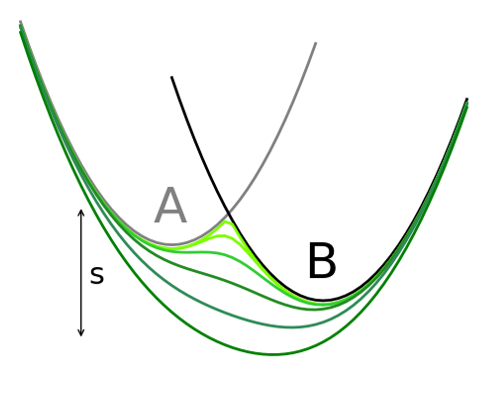
\includegraphics[width=\textwidth]{fig/intro/EDS_parmeters_s.png}
        \caption{Effect of $s$ on $V_R$}
        \label{fig: EDS_potential_behavioura}
    \end{subfigure}
    \begin{subfigure}{0.44\columnwidth}
        \centering
        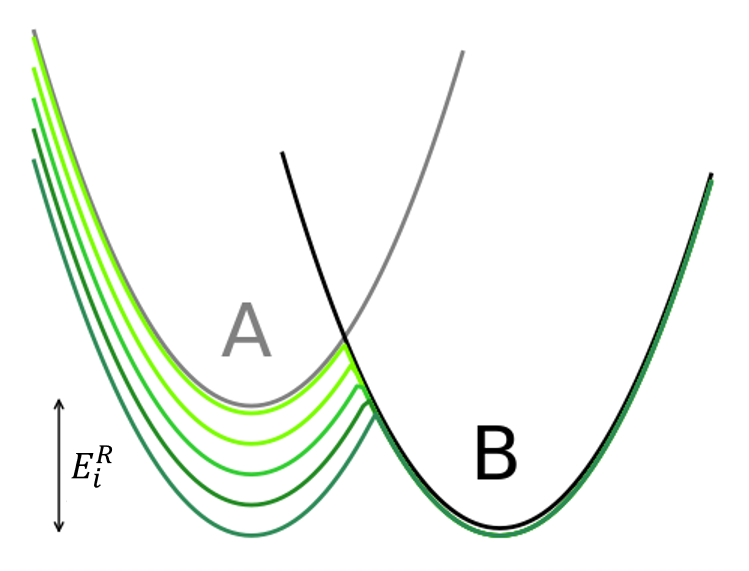
\includegraphics[width=\textwidth]{fig/intro/EDS_parmeters_Eoff.png}
        \caption{Effect of $E_i^R$ on $V_R$}
        \label{fig: EDS_potential_behaviourb}
    \end{subfigure}
    \end{center}
    \caption{Schematic illustration of the effect of the two types of EDS reference-state parameters. (\textbf{A}): The smoothing parameter $s$ decreases the barriers between the end states. If $s$ is too small, an ``undersampling'' situation occurs with a global unphysical minimum. (\textbf{B}): The energy offsets $\textbf{E}^R$ provide equal weighting to all end states in the EDS reference state.  The figure was generated with Ensembler\cite{Ries2021} (Chapter \ref{ch:feens}).}
    \label{fig: EDS_potential_behaviour}
\end{figure}

% laws of motion of R
The force on a particle $k$ in the EDS reference state is calculated as \cite{Christ2008},
\begin{equation}
    \textbf{f}_k(t)=-\frac{\partial V_R(\textbf{r}; s, \textbf{E}^R)}{\partial \textbf{r}_k} = \sum^N_{i=1}\frac{e^{-\beta s(V_i(\textbf{r}) -E_i^R)}}{\sum^N_{j=1}{e^{-\beta s (V_j(\textbf{r})-E_j^R)}}}  \left( -\frac{\partial V_i(\textbf{r})}{\partial \textbf{r}_k} \right) \,.
    \label{eq:laws_of_motion}
\end{equation}
%
For $s$ values close to one, the reference-state forces are dominated by the one end state, for which the current coordinates are most favourable, while the other end states give high energies and therefore contribute little (i.e. ``dummy states'').  
For small $s$ values (undersampling situation), all end states contribute effectively to the forces, resulting in the global unphysical minimum.

%% ddFE
The free-energy difference between two end states $A$ and $B$ can be calculated by employing the Zwanzig equation twice forming a path via the reference state~$R$ \cite{Zwanzig1954,Christ2007,Christ2008},

\begin{align} \nonumber
    \Delta G_{\text{BA}} &=  \Delta G_{\text{BR}} + \Delta G_{\text{RA}} \\ 
    &=-\frac{1}{\beta}\left(\ln \langle e^{-\beta (V_B-V_R)}\rangle_R - \ln \langle e^{-\beta (V_A-V_R )}\rangle_R\right) \\ 
    &= -\frac{1}{\beta} \ln \frac{\langle e^{-\beta (V_B-V_R)}\rangle_R}{\langle e^{-\beta (V_A-V_R)}\rangle_R}.
    \label{EQ: Free Energy calculation via reference state}
 \end{align}

%---------------------------
\FloatBarrier

\subsection{Replica-Exchange EDS (RE-EDS)}
The recently introduced RE-EDS method \cite{Sidler2016,Sidler2017} is a type of Hamiltonian replica exchange \cite{Hansmann1997,Sugita2000} with the smoothness parameter $s$ as the exchange dimension ($1 \geq s > 0$), which was inspired from constant pH simulations by Lee \textit{et al.} \cite{Lee2014,Lee2015}. The approach is shown schematically in Figure \ref{fig:RE-EDS_Scheme}.
RE-EDS does not require a single (optimal) $s$-value. Instead enhanced sampling is achieved by exchanging between the replicas with different smoothness levels. This simplifies the parameter choice problem and thus, the method can be applied to systems with more than two end states \cite{Sidler2016,Sidler2017}.

%Exchange criterium
For the pairwise exchanges between neighboring replicas $k$ and $l$, a Metropolis-Hastings criterion \cite{Hastings1970} is used \cite{Sidler2016,Sugita2000},
\begin{equation}
    \begin{split}
    p_{k,l} = min\bigg(1, \exp \Big[
                &-\beta \big((H_{R}(\textbf{r}_k; s_l)+H_{R}(\textbf{r}_l; s_k))\\
                &-(H_{R}(\textbf{r}_l; s_l)+H_{R}(\textbf{r}_k; s_k))\big)  \Big] \bigg) ,
    \end{split}
\end{equation}
where $H_{R_k}$ and $H_{R_l}$ are the reference-state Hamiltonians of the respective replicas, $\textbf{r}_k$ and $\textbf{r}_l$ are the current coordinates of the replicas.

Replicas are placed between $s=1.0$ and a lower bound of $s$, where the reference state is in undersampling. The replicas with low $s$ values facilitate the transitions between the low-energy regions of the  different end states. Especially for systems with slowly adapting environments (e.g. protein binding pockets), regions in $s$-space with very low acceptance probability can occur. Thus, to ensure sufficient exchanges between all pairs of replicas, a local variant of the round-trip time optimization algorithm \cite{Katzgraber2006, Nadler2008} was developed to optimally place the replicas in $s$-space \cite{Sidler2017}.
It was found that a single set of energy offsets can be used for all replicas \cite{Sidler2016}. However, it is important that these energy offsets are chosen well to avoid ``leakage'' effects, resulting in one or more end states not being properly sampled \cite{Sidler2016}.
The final free-energy differences are estimated from the replica at $s=1.0$, which represents the physical minima of the end states.

\begin{figure}[h]
    \centering
    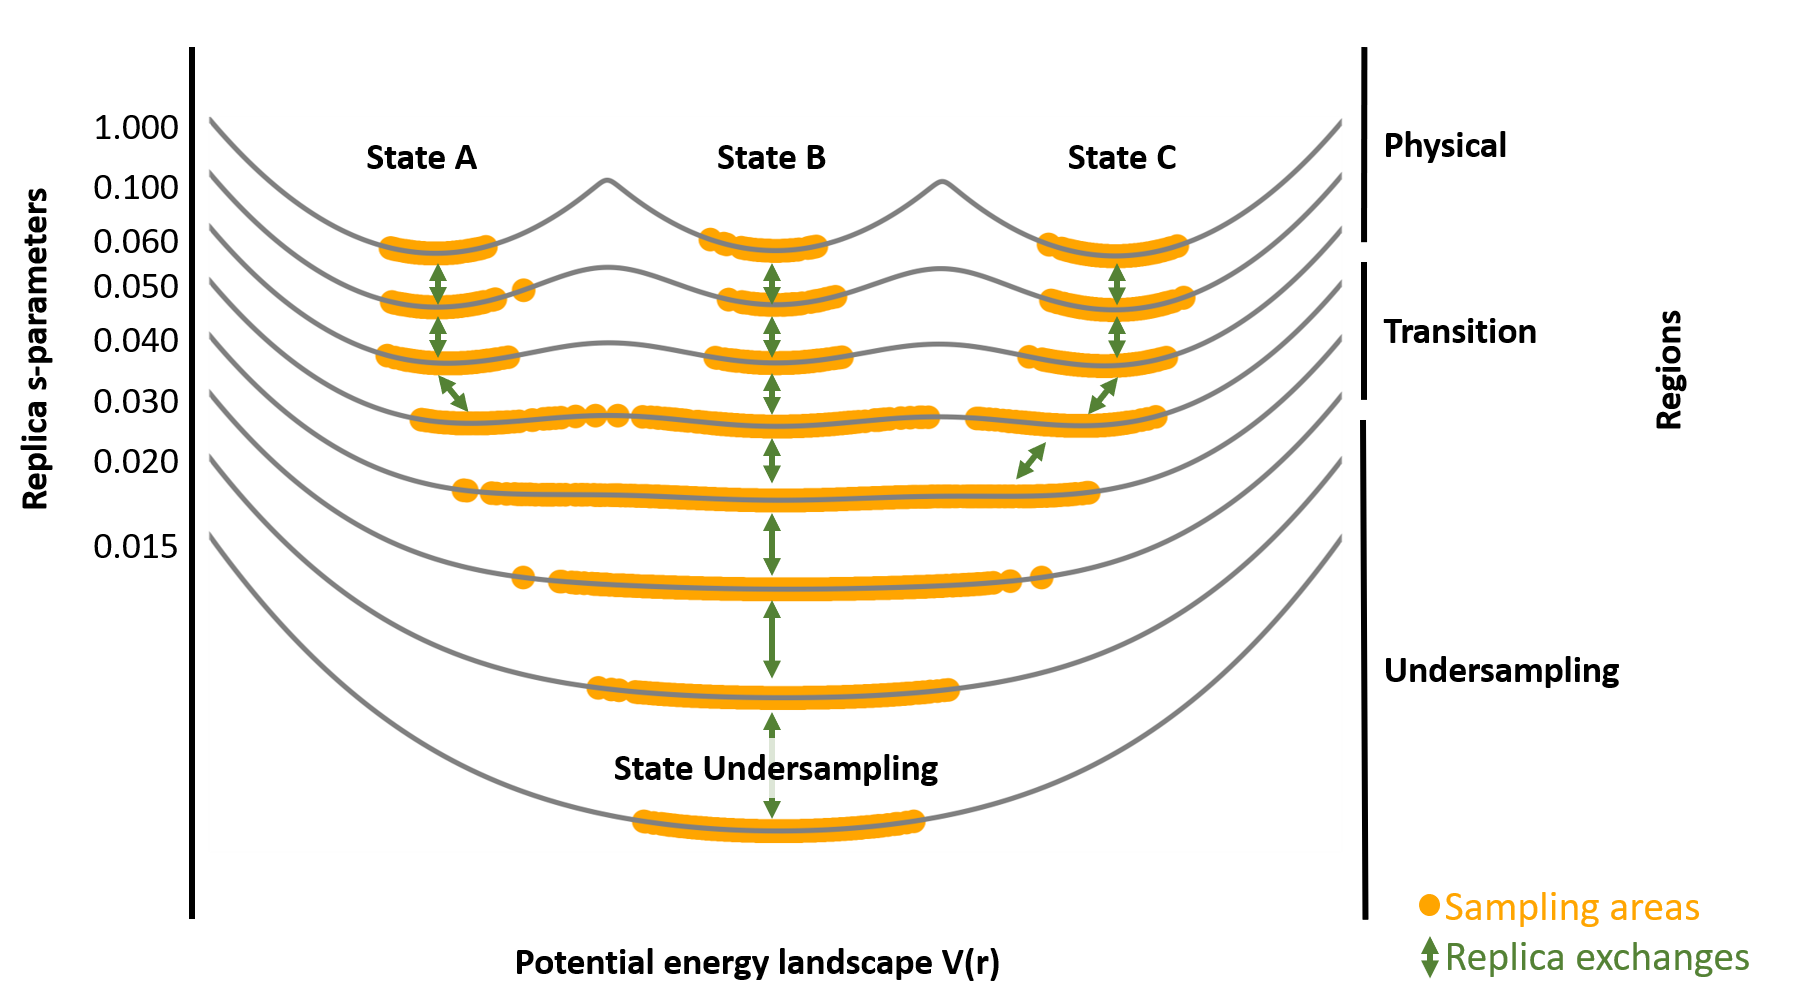
\includegraphics[width=\columnwidth]{fig/theory/Reeds_scheme_first.png}
    \caption{Schematic illustration of RE-EDS with three harmonic oscillators as end states ($A$, $B$, and $C$). Each replica differs by the $s$-parameter, generating reference states with a different degree of smoothness. Sampling of each replica is denoted with orange dots. Exchanges between the replicas are indicated with green arrows. The replica graph shows three regions: a ``physical'' region where $s$ is close to 1, a transition region, and the ``undersampling'' region when $s$ approaches zero. The figure was generated with Ensembler \cite{Ries2021}  (Chapter \ref{ch:feens}).}
    \label{fig:RE-EDS_Scheme}
\end{figure}

%---------------------------
\FloatBarrier

\subsection{Automatic Parameter Optimization}
To facilitate the determination of the energy offsets and $s$-parameter distribution, we have extended and further automatized the previous \cite{Sidler2017} RE-EDS workflow (Figure \ref{fig:Workflow}).
\begin{figure}[h!]
    \centering
    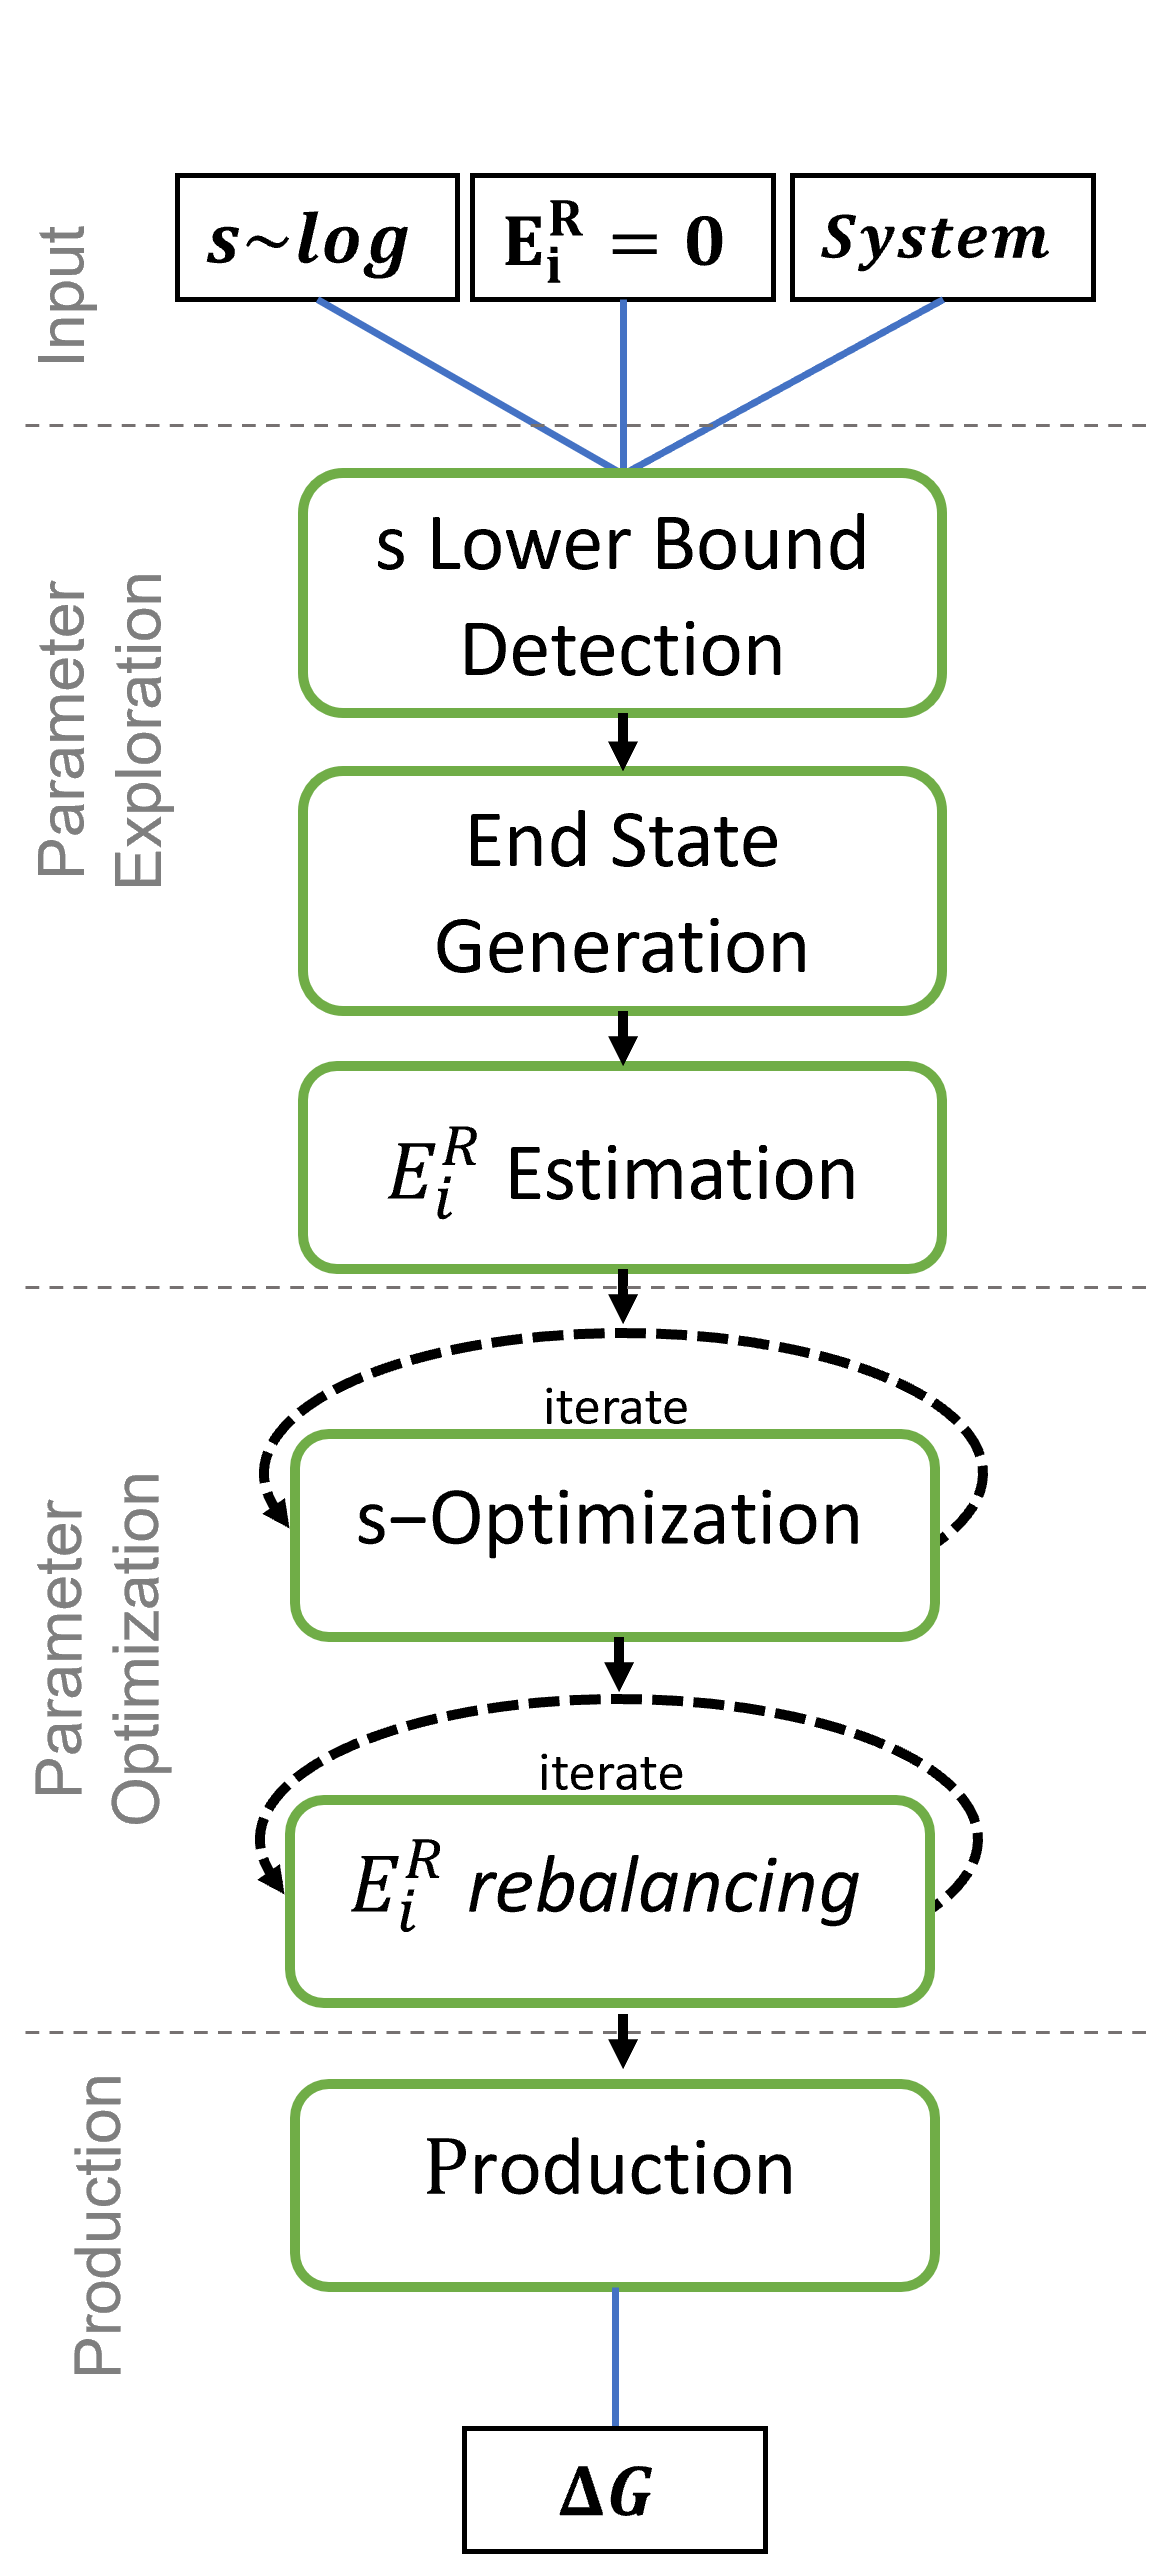
\includegraphics[width=0.5\columnwidth]{fig/theory/RE_EDS_Pipeline.png}
    \caption{The RE-EDS workflow can be split into four steps: (1) Input stage with energy offsets set to $E_i^R=0$ and a set of $s$-parameters logarithmically distributed between $1$ and $10^{-5}$; (2) Parameter exploration to determine the lower bound for $s$, to obtain equilibrated coordinates for each end state, and to estimate initial energy offsets with the PEOE scheme \cite{Sidler2016}; (3) Parameter optimization to improve the $s$-distribution with the N-LRTO algorithm \cite{Sidler2017} and the state sampling with energy offset rebalancing; (4) Production run and calculation of the free-energy differences.}
    \label{fig:Workflow}
\end{figure}

%
The initial input for a system with $N$ end states consists of a prepared EDS system (i.e. topology,  perturbation topology, initial coordinates, and distance restraints), a list of energy offsets of length $N$ with $E_i^R = 0; ~ \forall ~ i \in [1,...,N]$, and a list of $s$-parameters, which are logarithmically distributed in the range $s_i \in [1, 10^{-5}]$. Typically, we use 21 initial $s$ values. 

The parameter exploration consists of three substeps: (i) determining the lower bound for the $s$-distribution (newly introduced), (ii) obtaining optimized coordinates within the EDS set-up for each end state (newly introduced), and (iii) estimation of an initial set of energy offsets (as done previously in Ref.~\citenum{Sidler2016}).

%%1. initial parameter search
To enable sampling of all end states at $s=1.0$, some replicas have to be in undersampling to facilitate transitions. However, for efficiency reasons (and numerical stability) the number of replicas $M$ in undersampling should be small and the lowest $s$-value should be as high as possible. From a short simulation with the initial $s$-distribution between $[1, 10^{-5}]$, the highest smoothing parameter $s_{M_\mathrm{us}}$ at which undersampling still occurs is determined and used in the following as a lower bound for the $s$-distribution. The $s$-distribution for the next step is then defined by logarithmically distributed replicas between $s=1.0$ and the automatically determined lower bound.

%%%state optimization
Optimized coordinates for each end state in the EDS setup can be automatically obtained by short parallel simulations, where one end state in turn is favoured by setting an arbitrarily large energy offset for this state. 
The optimized coordinates allow the user to start RE-EDS simulations from different end states and are needed for the subsequent parameter optimization. 

 %%% estimate EOFFs:
In the last substep, $E_{\text{i}}^{\text{R}}$ estimation, the previously developed parallel energy offset estimation (PEOE) \cite{Sidler2016} scheme is used to estimate the initial set of energy offsets. This is done based on a short simulation with the initial parameters. For each replica $k$ in the undersampling region, the energy offsets are extracted using \cite{Sidler2016},
\begin{equation}
    E_{i}^{R}(new)=-\frac{1}{\beta}\ln \Big < e^{-\beta \big(V_i(\textbf{r})-V_R(\textbf{r}; s_{k},\textbf{E}^{R}(old))\big)}\Big>_{R(s_{k},\textbf{E}^{R}(old))} .
    \label{eq: EoffEstimator}
\end{equation}
The energy offsets that were extracted in parallel for the $k$ replicas are subsequently averaged and used as initial set of energy offsets. These energy offsets should provide a first solution that is close to the optimal choice of energy offsets, which leads to an optimal state sampling of all end states in the RE-EDS simulation. As the initial energy offsets are obtained from the replicas in undersampling, they may not be exactly optimal and require fine-tuning in the next phase. 


%%2. optimization of parameters
In the second step of the RE-EDS workflow, first the $s$-distribution is optimized and subsequently the energy offsets are fine tuned.
%
%%% s-Optimization:
The $s$-distribution is improved by minimizing the round-trip time $\tau$ and increasing the number of round-trips, using the multistate local round-trip time optimization (N-LRTO) algorithm \cite{Sidler2017}. The optimization is performed in an iterative manner with short simulations.
This step is required as exchange bottlenecks between two replicas might occur leading to a very slow round trip time or to no round trips at all. 
In the N-LRTO algorithm, new replicas are inserted in each iteration by linear interpolation in the $s$-regions with exchange bottlenecks, while the replica positions of the previous iteration are retained. Adding replicas theoretically increases the round-trip time because of a longer path between the top and bottom replicas. However, the addition of intermediate replicas also increases the exchange probability between neighboring replicas, thus reducing the round-trip time. With the optimization algorithm, we aim to determine the balance between the length of the replica path and the likelihood of exchange between replicas for minimal round-trip time. The exchange bottlenecks are identified for each end state separately (i.e. multistate). The number of replicas added can be chosen by the user. The iteration is stopped when the average round-trip time $\overline{\tau}$ converges. 
The N-LRTO variant is needed for systems for which severe bottlenecks are observed with the initial logarithmic $s$-distribution (e.g. protein binding pockets). For systems with smaller perturbations, the global multistate variant (N-GRTO) \cite{Sidler2017} can be more efficient as this algorithm re-distributes the replicas in $s$-space according to the exchange statistics. %In very severe cases, this can lead to an oscillating behavior, as one bottleneck is fixed, but another appears due to an imbalance of replica shifting.
%
In this study, we started with the same number of replicas as used for the PEOE scheme above and added four replica positions per iteration in the N-LRTO algorithm.

%%%% Eoff Rebalancing:
After optimizing the number of round trips and $\tau$, the distribution of the state sampling is improved. To reach the ideal situation that each end state is sampled to an equal amount, the initial energy offsets need to be fine tuned, while keeping the round trips approximately constant. For this, we introduce here the energy offset rebalancing scheme.
To avoid overshooting, a correction factor is calculated and applied iteratively,
\begin{equation}
    \Delta E^{corr}_i = - \frac{1}{\beta} \ln \left( \frac{f_i^{\text{mc}}+c}{f^{\text{mc,ideal}}_{i}+c} \right),
    \label{eq: EoffRebalancing}
\end{equation}
where $f_i^{\text{mc}}$ is the current sampling fraction (or estimated probability) of an end state contributing to $V_R $, and $f^{\text{mc,ideal}}$ is the ideal sampling fraction (see Section \ref{metrics}). 
%
To make the approach more robust, a pseudo count $c$ is introduced to avoid singularities with zero sampling, which is defined as,
\begin{equation}
    c = \frac{f^{\text{mc,ideal}}}{x},
    \label{eq: EoffRebalancingPseudoCount}
\end{equation}
with the intensity factor $x$.
The default of the pseudo count was chosen to result in a maximal correction of $\Delta E^{corr}_i=8.43$~kJ/mol, corresponding to a minimum 30-fold reduced sampling compared to the expected optimal sampling.

%%% 3. production run
After optimizing the RE-EDS parameters, the production run is performed for a chosen length. 
The free-energy differences are subsequently calculated using the replica at $s=1.0$ with Eq.~(\ref{EQ: Free Energy calculation via reference state}).

\subsubsection{Starting State Mixing}
The sampling in RE-EDS simulations can be further improved by using starting coordinates for the replicas corresponding to the different end states (i.e. replica 1 starts in a low-energy configuration for end state 1, replica 2 in a low-energy configuration for end state 2, etc.). This technical approach is called ``starting state mixing'' (SSM) in the following and is also used for Hamiltonian replica-exchange TI calculations (see e.g. \citenum{Graf2016, Hahn2020}). The optimized coordinates obtained in the parameter exploration step can be used for SSM. We compare RE-EDS simulations with SSM and with a single set of starting coordinates (abbreviated as 1SS).  

\subsubsection{Analysis}
\label{metrics}
Three types of metrics were used to quantify the sampling in RE-EDS simulations. The first metric determines for each end state $i$ the sampling fraction where it is maximally contributing to the reference state, i.e. $f_i^{\text{mc}}$. A maximally contributing state is defined as the end state with the lowest potential energy minus its energy offset in a frame. As can be seen in  Eq.~\eqref{eq:laws_of_motion}, maximally contributing end states have the largest impact on the reference-state sampling at a given time point.

%
Optimal sampling in a RE-EDS system is achieved when all end states are sampled as maximally contributing states to an equal extent at $s=1.0$, i.e. 
\begin{equation}
f_{i}^{\text{mc,ideal}} = \frac{1}{N} ~, \forall ~ i~\in~ \{1, ..., N\}
\label{eq: optimalDominationSamplingDist}
\end{equation}

The second metric is the estimated sampling fraction of ``physical occurrence'' of an end state $i$, i.e. $f_i^{\text{occur}}$. As a result of phase-space overlap with the current maximal contributing end state, other end states in the EDS system might be sampled simultaneously. An end state is counted as ``occurred'' when its potential energy is below the threshold $V_i \leq T_{i}^{\text{phys}}$ at a time point $t$. 
These thresholds are estimated during the second substep of the parameter exploration phase. If end states show no phase-space overlap, $f_i^{\text{occur}}$ will be (nearly) the same as $f_i^{\text{mc}}$. 

Undersampling is detected with a third metric using the thresholds $T_{i}^{\text{us}}$. These thresholds are determined in the first substep of the parameter exploration phase from the simulation with the lowest $s$-value. If all end states have a potential energy below their respective $V_i - E^R_i \leq T_{i}^{\text{us}}$, the current frame is characterized as undersampling. \cite{Sidler2016} 

\FloatBarrier

%================================================================================
\section{Computational Details}
%================================================================================

In the computational studies, two pairs of structurally similar cyclic peptides were selected, i.e., Nleu-5R/Nleu-5S and Nleu-2R/Nleu-2S (Figure \ref{fig:permCMols}). 
The first pair presents a ``permeability cliff'', i.e., the two peptides show a large difference in the passive permeability in the PAMPA assay (Nleu-5R: $−log(P_e)$~=~5.4; Nleu-5S: $−log(P_e)$~=~7.2), despite a high structural similarity. 
In contrast, the second pair is similar in both structure and permeability (Nleu-2R: $−log(P_e)$~=~6.1; Nleu-2S: $−log(P_e)$~=~5.8). 
For each of these four peptides, $250$ starting coordinates were generated using the macrocycle variant of the OMEGA conformer generator from OpenEye. \cite{Hawkins2012, Hawkins2010, Poongavanam2018}
Conformers were energy-minimized for maximum $2000$ steps with the steepest descent \cite{Ruder2016} approach using the GROMOS software package \cite{Schmid2012} with the GROMOS 54A7 force field. \cite{Schmid2011} 
Each minimized starting conformation was solvated in a cubic box of simple-point-charge (SPC) water \cite{Berendsen1981} (on average, $4172$ solvent molecules) or chloroform \cite{Tironi1994} (on average, $980$ solvent molecules). 
For each system, an MD simulation of $101~$ns length was performed under isothermal–isobaric (NPT) conditions with the leap-frog integration algorithm \cite{Hockney1970, Gunsteren1988} and a time step of $2$~fs. 
The first 1 ns was discarded as equilibration. Bond lengths were constrained with SHAKE \cite{Ryckaert1977} and a tolerance of $10^{–4}$~nm. 
Nonbonded interactions were calculated using a twin-range scheme with a short-range cutoff of $0.8$~nm and a long-range cutoff of $1.4$~nm. 
The electrostatic nonbonded contributions beyond the long-range cutoff were calculated with the reaction-field \cite{Tironi1995} approach, setting the dielectric permittivity to 61.0 \cite{Heinz2001} for water, and to 4.8 \cite{Tironi1994} for chloroform. 
The temperature was kept constant at $300$~K using the weak coupling scheme \cite{Berendsen1984} and a coupling time of $0.1~\text{ps}^{–1}$. 
The pressure was kept at $1.031$~bar ($1$~atm) with the same type of algorithm, a coupling time of $0.5~\text{ps}^{–1}$, and an isothermal compressibility of $0.001654~\text{bar}^{–1}$ for chloroform and $0.0004575~\text{bar}^{–1}$ for water. 
Translational motion of the center of mass of the simulation box was removed every $2$~ps. Energies and coordinates were written every $5$~ps.

Trajectory analysis was performed with PyEmma \cite{Scherer2015} and MDTraj \cite{Mcgibbon2015}. 
The selection of features for the structural clustering consisted of the distances between all pairs of polar atoms and the backbone torsional angles, resulting in total $57$ features. 
This selection was reduced to three to five dimensions (depending on the peptide) with TICA \cite{Molgedey1994} using a cumulative variance of $0.9$ as criterion and a TICA correlation lag time of $50$~ps. 
Based on these TICs, the frames were clustered with a common nearest neighbor (CNN) algorithm \cite{Keller2010, Weiß2021} using a cutoff of $0.2$ and a similarity of $20$. 
Comparison of selected clusters with NMR experiments was performed with the GROMOS++ package of programs. \cite{Eichenberger2011}
The coefficients for the Karplus curve were taken from Vögeli \textit{et al.} \cite{Voegeli2015}
Analysis of hydrogen bonds and torsional angles was performed with MDTraj. 
The 3D-PSA was calculated with our implementation \cite{Witek2019} of the workflow in Ref.~\citenum{Tyagi2018} using PyMol \cite{Delano2020}.
Statistical analysis of all results was carried out using the Python packages Pandas, NumPy and SciPy.\cite{Virtanen2020}



%================================================================================
\section{Results and Discussion}
%================================================================================

The chosen model system of five inhibitors of CHK1 kinase exemplifies different core-hopping transformations (i.e. ring size change, ring opening/closing, ring extension) and R-group modifications \cite{Wang2017}, increasing the complexity compared to the systems previously studied with RE-EDS. Furthermore, the performance can be directly compared to the results obtained with FEP+ and OPLS3 in Ref.~\cite{Wang2017} as well as with QligFEP results in Ref.~\cite{Jespers2019}.

\subsubsection{Parameter Exploration and Parameter Optimization}
The RE-EDS workflow was started by estimating the lower bound for the $s$-distribution. Using the above mentioned undersampling criterion (see Methods section), a lower bound of $s=0.01$ was determined for the protein-ligands complex and $s=0.0056$ for the ligands in water. 

%State Optimizations
Optimized coordinates were obtained for all five ligands, as verified by comparing the potential-energy distribution from the EDS simulation with the one extracted from a standard MD simulation of the respective ligand (Figure S1 in the Supporting Information). % SUPPL
From these same steps, the potential-energy thresholds for the occurrence sampling ($T_{i}^{\text{phys}}$) and undersampling ($T_{i}^{\text{us}}$) were estimated.

%Eoff:
The energy offsets $\vec{E}^R$ were estimated from a short RE-EDS simulation with the PEOE \cite{Sidler2016} scheme and are listed in Table \ref{tab:CHK1_set2_Eoff}.
For $s=1.0$, the energy offsets should ideally be equal to the free energy of the corresponding state (i.e. $\Delta E^R_{ji} = \Delta G_{ji}$) such that the partition function of the reference state is the sum of the partition functions of the end states \cite{Christ2008}. Therefore, the comparison between the relative estimated energy offsets in water and in complex ($\Delta \Delta E^R_{ji} = \Delta E^R_{ji,\text{complex}} - \Delta E^R_{ji,\text{water}}$) and the relative binding free energy $\Delta \Delta G^\text{bind}_{ji}$ can be used to (roughly) assess the quality of the estimated energy offsets. As shown in Figure S2 in the Supporting Information, % SUPPL
the energy offsets estimated from the SSM simulations are in better agreement with the experimental relative binding free energies than those estimated from the 1SS simulations.

\begin{table}[h]
\caption{Energy offsets $\vec{E^R}$ estimated from a short RE-EDS simulation using the PEOE \cite{Sidler2016} scheme. The errors indicate the standard deviation over the different replicas in undersampling. All energy offsets were calculated relative to ligand L1. The starting coordinates were selected following the 1SS or the SSM approach (see Theory and Methods sections).}
\label{tab:CHK1_set2_Eoff}
\resizebox{\columnwidth}{!}{%
\centering
\begin{tabular}{ l | r r | r r }
 Ligand & \multicolumn{2}{c|}{Water}&\multicolumn{2}{c}{Complex}  \\ 
  &RE-EDS 1SS [kJ~mol$^{-1}$]&RE-EDS SSM [kJ~mol$^{-1}$]&RE-EDS 1SS [kJ~mol$^{-1}$]&RE-EDS SSM [kJ~mol$^{-1}$]\\ 
 \hline
     L1 & $0.0$ & $0.0$ & $0.0$ & $0.0$ \\ 
     L17 & $11.07 \pm 7.61 $ & $17.81 \pm 0.69 $ & $20.03 \pm 5.04 $ & $18.19 \pm 3.43$ \\
     L19 & $-9.38 \pm 6.85 $ & $ -12.37 \pm 5.23 $ & $-2.09 \pm 1.56 $ & $ 2.4 \pm 1.56$ \\
     L20 & $-53.15 \pm 2.95 $ & $ -56.01 \pm 13.67 $ & $ -58.73 \pm 4.87 $ & $-52.2 \pm 2.6$\\
     L21 & $-76.75 \pm 5.79 $& $-69.15 \pm 3.74 $ & $ -77.29 \pm 3.12 $ & $ -77.9 \pm 3.4$\\
\end{tabular}
}
\end{table}

%S-Optimization
The optimization of the $s$-distribution was performed with the N-LRTO \cite{Sidler2017} algorithm, thereby minimizing the average round-trip time $\overline{\tau}$ in the replica graph. For the 1SS complex system, four optimization iterations were used. For the other systems, three iterations were used. 

%
In the first iteration, the total number of observed round trips was very low or zero for all approaches. In the following iterations, this quantity increased, and the average round-trip time decreased for all simulations (Figure \ref{fig: CHK1_RingOpening_sOptimization}). The number of round trips was generally smaller in the complex than in water due to a more pronounced gap region \cite{Sidler2017}.
Already after the second iteration, the round-trip time was reduced in all approaches. The improvement of the $\overline{\tau}$ over the iterations can also be seen in Figure S3 in the Supporting Information. % SUPPL
%% s-replica placements
As can be seen in the third row of Figure \ref{fig: CHK1_RingOpening_sOptimization}, the optimization algorithm increases the density of the replicas around $s = 0.041$, where the major gap region lies.

\begin{figure}[h]
\centering
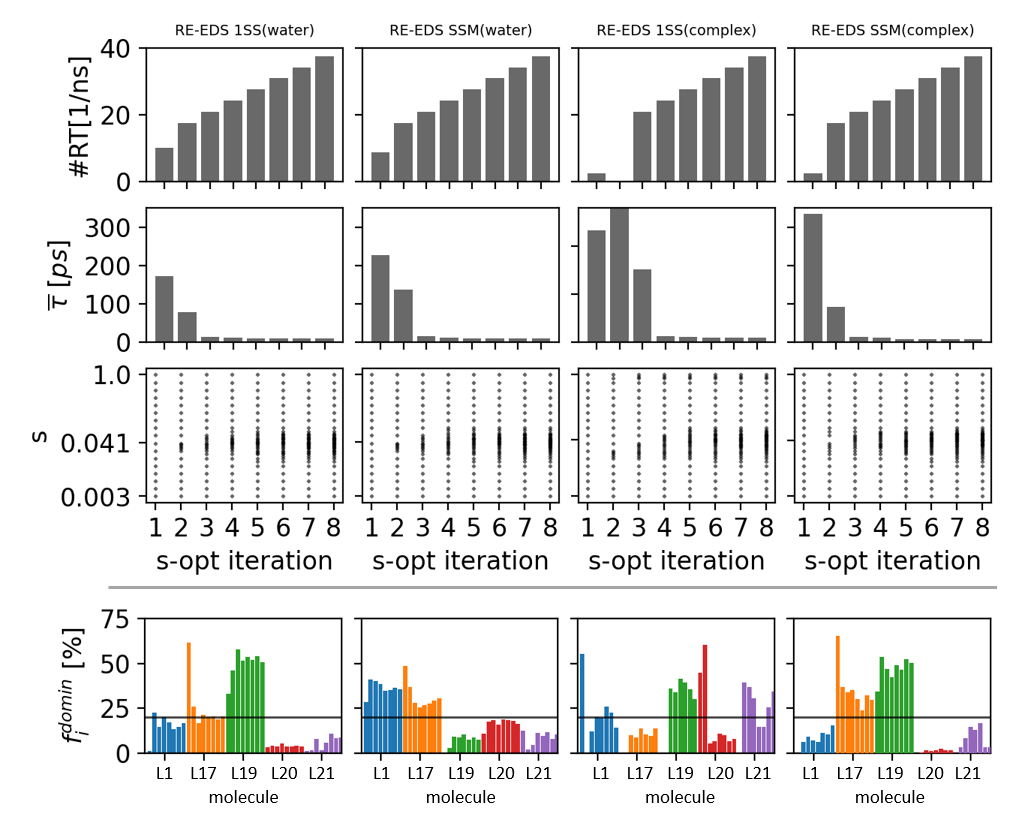
\includegraphics[width=\textwidth]{fig/results/ringOpening/paramOptimization/S-optimization_ringOpening.png}
\caption{Optimization steps of the $s$-distribution with the N-LRTO \cite{Sidler2017} algorithm followed by the energy offset rebalancing scheme (start indicated by the red horizontal line). The measured quality criteria were the number of round trips (1. row), the average round-trip time $\overline{\tau}$ (2. row), the placement of the replicas in $s$-space (3. row), and the sampling fractions of maximally contributing states $f_{i}^{\text{mc}}$ (4. row). The light colored bars of $f_{i}^{\text{mc}}$ indicate $s$-optimization iterations, whereas the fully colored bars indicate energy offset rebalancing steps. }
\label{fig: CHK1_RingOpening_sOptimization}
\end{figure}



%% tau converge - Conclusion
The $s$-optimization was stopped after a sufficiently high number of round trips and low round-trip time was reached. 
This resulted in 20 replicas for the ligands in water after three $s$-optimization iterations.
For the protein-ligands complex, the fourth $s$-optimization iteration was chosen for the 1SS approach, and the third iteration for the SSM approach, resulting in 29 and 25 replicas, respectively. 
The average round-trip time after convergence was $\overline{\tau} = 0.4 \pm 0.2$~ns for all simulations.

After the $s$-optimization, the energy offset rebalancing scheme was applied to improve the state sampling. 

%RT analysis
During the rebalancing steps, no further replicas were added to the $s$-distribution. It is essential for the success of the rebalancing scheme that round trips occur. Therefore, the number of round trips and average round-trip time were monitored. In all systems, the number of round trips and $\overline{\tau}$ remained relatively stable over the four rebalancing steps. For the RE-EDS 1SS approach in water, the number of round trips slightly decreased but never dropped to zero.

%% states sampling
Across the optimization steps, also the sampling of the end states as maximally contributing states at $s=1.0$ was monitored.
During the $s$-optimization, some end states ``vanish'' and are no longer sampled as maximal contributing states. This leakage effect can occur when the initially estimated $E^{\text{R}}$ are not exactly optimal \cite{Sidler2016}. 
With energy offset rebalancing, the sampling of each end state can be recovered, and the sampling distribution approaches the ideal case.
%After the s-optimization the MAE($P^{\text{maxContrib}}$) was for all approaches approximately at $25\%$, with the exception of the 1SS water system, here it was $20\%$. 
After rebalancing, all end states showed a $f_i^{\text{mc}} > 0$ and the mean absolute deviation of the sampling distribution from ideal decreased from $20-25\%$ to approximately $7-12\%$ (Figure S4 in the Supporting Information). % SUPPL
 
\subsection{Free-Energy Calculation}
After successfully optimizing the RE-EDS parameters, the production runs were performed for $3.5$~ns. 

%%Sampling++
Both in water and in complex, the potential-energy distributions of the end states generally match well the corresponding distributions from the standard MD simulations of the single end states (Figure \ref{fig:RingOpening_sampling_comparison}). Only in the complex 1SS approach, a deviation can be seen for L17, with a slight shift to higher potential energies. This is due to insufficient sampling of L17 in this case (see below). 
%
The analysis of the maximally contributing end states at $s=1.0$ shows that in water all end states were sampled close to the ideal equal distribution (Figure S5 in the Supporting Information). % SUPPL
In the simulation of the protein-ligands complex, there are still differences in sampling. Especially with the 1SS approach, L19 is generally sampled too much, while L17 is not sampled enough. The situation is improved with the SSM approach.
Comparing $f_i^{\text{occur}}$ and $f_i^{\text{mc}}$ in Figure S5 indicates that the end states in the CHK1 system are clearly separated (i.e. no phase-space overlap). % SUPPL

\begin{figure}[h]
    \centering
    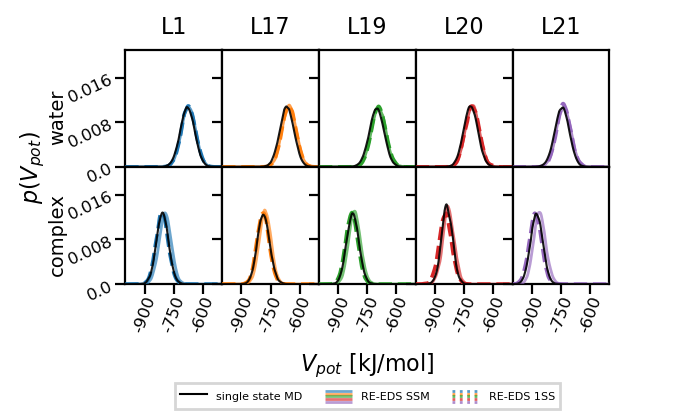
\includegraphics[width=\columnwidth]{fig/results/ringOpening/FE/RingClosure_system_final_sampling.png}
    \caption{Comparison of the Boltzmann reweighted potential-energy distributions obtained from standard MD simulations of a given end state (black) and from the RE-EDS production runs of the 1SS (green) and SSM (turquoise, dashed) approaches.}
    \label{fig:RingOpening_sampling_comparison}
\end{figure}

%%Accuracy
From the replica at $s=1.0$, the free-energy differences were calculated using Eq.~(\ref{EQ: Free Energy calculation via reference state}) and the resulting $\Delta \Delta G^\text{bind}_{ji}$ were compared with the experimental results taken from Ref.~\cite{Huang2012}. The results are shown graphically in Figure \ref{fig:CHK1_set2_FreeEnergyCalculation} and numerically in Table \ref{tab: RE-EDS_FE_RingCycleOpening_ddF}. The individual free-energy differences are given in Table S3 in the Supporting Information. %SUPPL
The RMSE with RE-EDS 1SS is $4.4$~kJ~mol$^{-1}$ and the MAE is $3.9\pm2.8$~kJ~mol$^{-1}$. 
%
%how I calculate the MAE and RMSD:
%MAE = np.mean(np.abs(ddG_differences))
%std(MAE) = np.std(np.abs(ddG_differences)) #gives an impression of absolute deviation of all ddG_diffs
%RMSE = np.sqrt(np.mean(np.square(ddG_differences))
%
The main deviations stem from ligand L17 in the RE-EDS 1SS approach, which can be explained by the insufficient sampling of L17 in the complex (see Figure \ref{fig:RingOpening_sampling_comparison} and Figure S5 in the Supporting Information). %SUPPL

The performance was substantially improved using the SSM approach with RE-EDS, giving an RMSE of $3.3$~kJ~mol$^{-1}$ and an MAE of $2.8 \pm 1.7$~kJ~mol$^{-1}$. 
Only two values (L21-L11) and (L21-L19) deviate more than $4.184$~kJ~mol$^{-1}$ (i.e. $1$~kcal~mol$^{-1}$) from experiment.
The Spearman correlation coefficient for RE-EDS 1SS is $r_{\text{Spearman}}=0.01$ and for RE-EDS SSM $r_{\text{Spearman}}=0.69$.

%%Performance:
Next, we assessed the convergence of the $\Delta G_{ji}$ values as a function of simulation time (Figure S6 in the Supporting Information). % SUPPL
For the RE-EDS 1SS approach, all free-energy differences appeared converged after $2.5$~ns in water and after $2.7$~ns in the complex. For the RE-EDS SSM approach, convergence was observed after $2.5$~ns in water and after $2.9$~ns in the complex.

\begin{figure}[h]
    \centering
    \begin{subfigure}{0.85\columnwidth}
        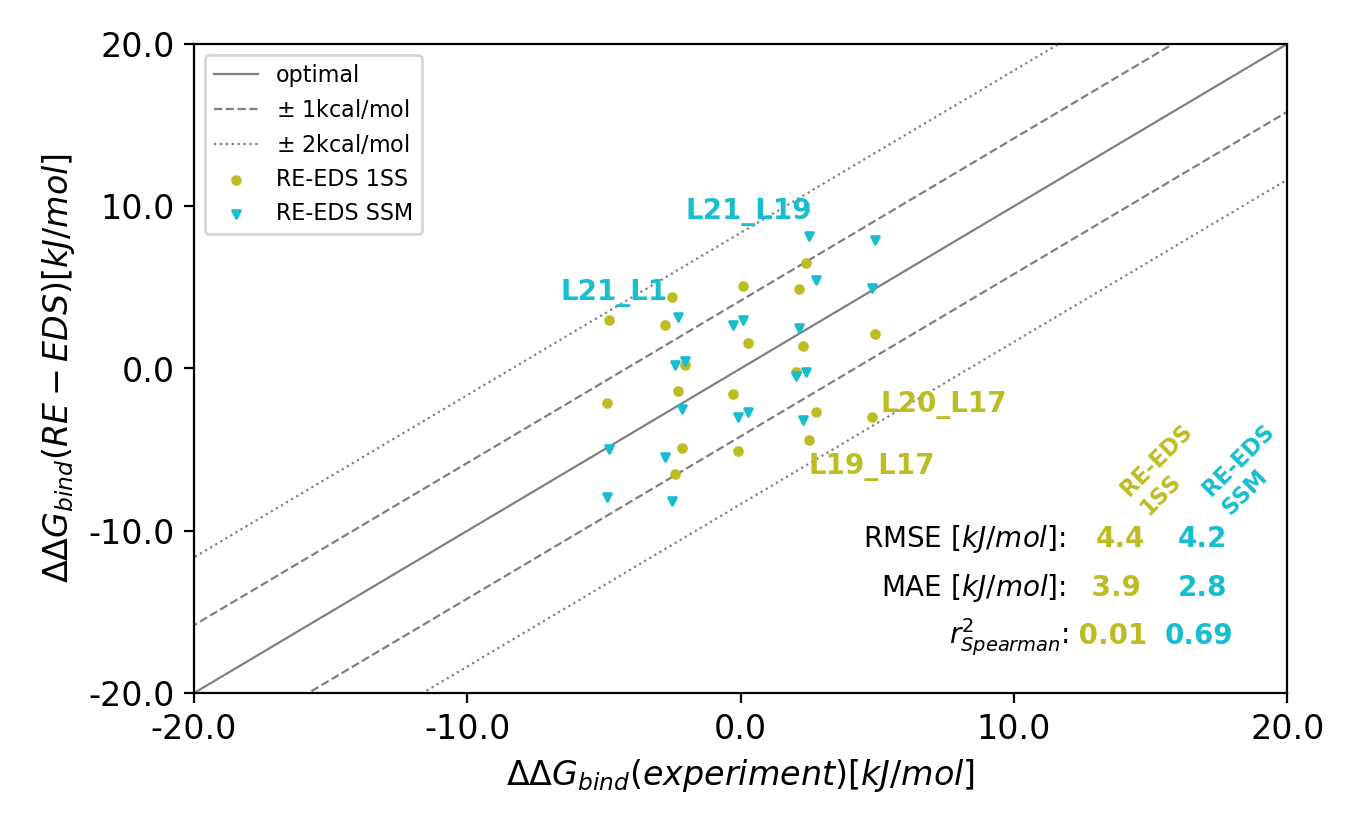
\includegraphics[width=\textwidth]{fig/results/ringOpening/FE/RingClosure_system_final_results_4ns_comparison.png}
        \end{subfigure}
    \begin{subfigure}{0.85\columnwidth}
        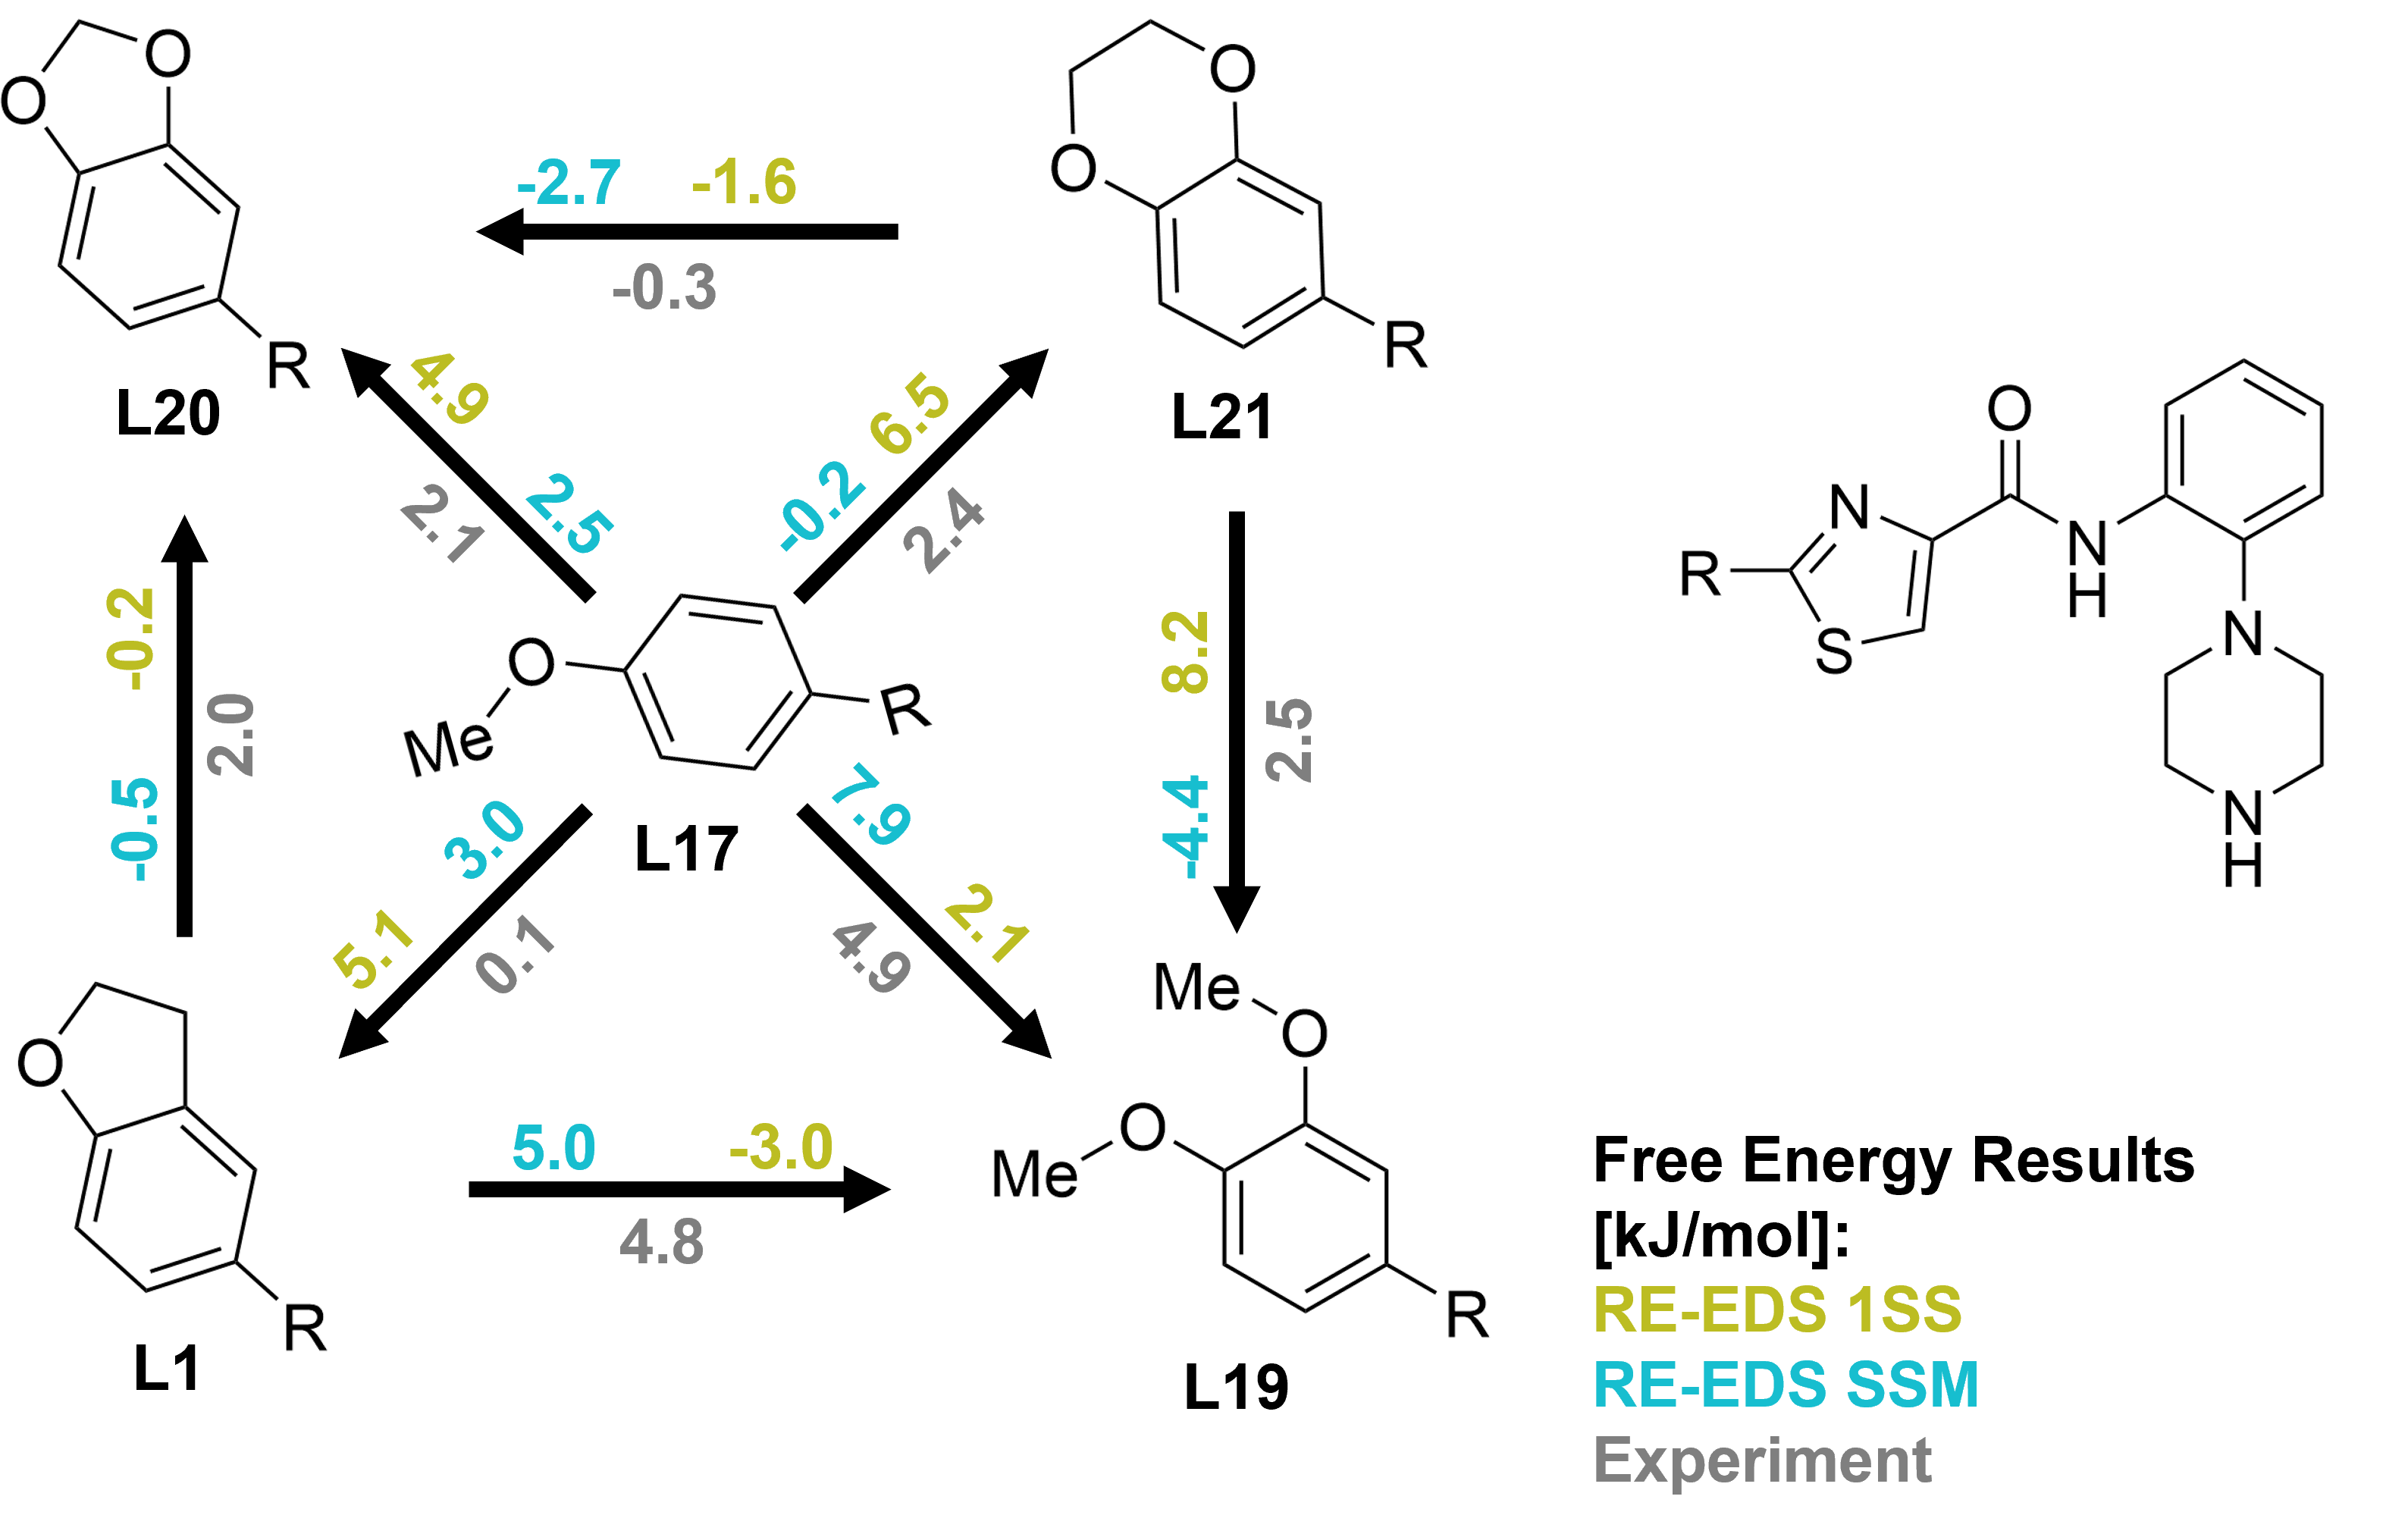
\includegraphics[width=\textwidth]{fig/results/ringOpening/FE/ddG_bind_paper_comparison_reeds_only_4nsSimulation.png}
        \end{subfigure}
    \caption{Free-energy differences estimated from the production run of $3.5$~ns length. (Top): Comparison between the experimental and calculated $\Delta \Delta G^\text{bind}_{ji}$ using RE-EDS 1SS and RE-EDS SSM. The results were calculated with all possible pairwise transformations (forward and backward). (Bottom): Graphical representation of the $\Delta \Delta G^\text{bind}_{ji}$ results with structures, inspired by the one in Ref.~\cite{Wang2017}.}
    \label{fig:CHK1_set2_FreeEnergyCalculation}
\end{figure}

%Comparison results with Schroedinger & Jespers
By applying the RE-EDS methodology to the same system of five CHK1 inhibitors as studied by Wang \textit{et. al.} \cite{Wang2017} and later on also Jespers \textit{et al.} \cite{Jespers2019}, a direct comparison with FEP+ and QligFEP is possible (Table \ref{tab: RE-EDS_FE_RingCycleOpening_ddF}). Note that the quality metrics were calculated over all possible pairs of ligands and in both directions, not only those directly calculated by FEP+ and QligFEP.
For FEP+, we obtained an RMSE of $2.4$~kJ~mol$^{-1}$ and an MAE of $1.8 \pm 1.2$~kJ~mol$^{-1}$ with a Spearman correlation coefficient of $r_{\text{Spearman}}=0.67$.
Including cycle closure correction (CC) \cite{Wang2017} reduced the RMSE to $2.1$~kJ~mol$^{-1}$ and the MAE to $1.9 \pm 1.0$~kJ~mol$^{-1}$. The Spearman correlation coefficient increased to $r_{\text{Spearman}}=0.73$.
Jespers \textit{et al.} \cite{Jespers2019} reported free-energy differences with QligFEP as an average over ten independent replicas, each with significantly less simulation time per $\lambda$-window than in Ref.~\cite{Wang2017}. For QligFEP, an RMSE of $2.3$~kJ~mol$^{-1}$, an MAE of $2.0 \pm 1.2$~kJ~mol$^{-1}$, and a Spearman coefficient of $r_{\text{Spearman}}=0.61$ was obtained.

Overall, the performance of RE-EDS SSM is comparable with the pairwise methods. The results with FEP+ CC and QligFEP showed a slightly higher accuracy compared to experiment, likely due to the different force fields used. The Spearman correlation coefficient is comparable with the other methods for the RE-EDS SSM approach.

\begin{table}[h]
\caption{Relative binding free energies $\Delta \Delta G^\text{bind}_{ji}$ from experiment and calculated with the RE-EDS 1SS and RE-EDS SSM approaches. For comparison, the results for FEP+ with and without cycle closure (CC) correction taken from Ref.~\cite{Wang2017} and the results for QligFEP taken from Ref.~\cite{Jespers2019} are listed. The free-energy differences of directly simulated paths were used to infer not directly simulated free-energy differences (marked in bold). If multiple indirect paths were possible, their average was used. The errors for QligFEP were determined in Ref.~\cite{Jespers2019} by calculating the standard deviation over ten replicas. For FEP+, the error of the results was taken from the used BAR \cite{Bennett1976} method and the FEP+ CC errors were obtained from the cycle closure analysis. For the RE-EDS approaches, the reported error is based on the statistical uncertainties of the $\Delta G_{ji}^{env}$ values estimated using Gaussian error approximation \cite{Christ2008}. The uncertainty estimate of the RMSE was obtained by a 100-fold bootstrapping approach. }
\begin{center}
\footnotesize
\resizebox{\columnwidth}{!}{%
\begin{tabular}{ c c |c |c|c|c|c|c}
  \multicolumn{2}{c|}{Ligands} & \multicolumn{1}{c|}{Exp. \cite{Huang2012}} &\multicolumn{1}{c|}{FEP+ \cite{Wang2017}}&\multicolumn{1}{c|}{FEP+ CC \cite{Wang2017}}&\multicolumn{1}{c|}{QligFEP \cite{Jespers2019}}&\multicolumn{1}{c|}{RE-EDS 1SS}&\multicolumn{1}{c}{RE-EDS SSM}\\ 
    $i$ & $j$  & [kJ~mol$^{-1}$]  & [kJ~mol$^{-1}$] & [kJ~mol$^{-1}$] & [kJ~mol$^{-1}$] & [kJ~mol$^{-1}$] & [kJ~mol$^{-1}$]  \\
  \hline
        L17 &  L1 &   0.1 & -3.6 $\pm$ 0.4          & -2.9 $\pm$ 1.0         & -1.6 $\pm$ 1.7                                     &    5.1 $\pm$ 0.8 &  3.0 $\pm$ 2.0 \\
        L19 &  L1 &  -4.8 & -3.9 $\pm$ 0.3          & -4.0 $\pm$ 0.6         & -1.7 $\pm$ 2.0                                     &    3.0 $\pm$ 1.0 & -5.0 $\pm$ 0.1\\
        L20 &  L1 &  -2.0 & -2.5 $\pm$ 0.1          & -3.1 $\pm$ 1.0         & -1.3 $\pm$ 1.3                                     &    0.2 $\pm$ 0.9 &  0.5 $\pm$ 0.1\\
        L21 &  L1 &  -2.3 &\textbf{-3.4} $\pm$ \textbf{0.7}  &\textbf{-3.2} $\pm$ \textbf{1.3} & \textbf{-0.1} $\pm$ \textbf{3.5} &   -1.4 $\pm$ 0.8 &  3.2 $\pm$ 0.1\\
        L19 &  L17 & -4.9 & -1.4 $\pm$ 0.3          & -1.1 $\pm$ 1.0         & \textbf{0.1} $\pm$ \textbf{2.6}                    &   -2.1 $\pm$ 0.6 & -7.9 $\pm$ 1.9\\
        L20 &  L17 & -2.1 &  0.3 $\pm$ 0.4          & -0.1 $\pm$ 0.8         & -1.3 $\pm$ 2.3                                     &   -4.9 $\pm$ 0.1 & -2.5 $\pm$ 1.9\\
        L21 &  L17 & -2.4 & -1.1 $\pm$ 0.4          & -0.9 $\pm$ 0.9         &\textbf{0.7} $\pm$ \textbf{2.6}                     &  -6.5 $\pm$ 0.1 &  0.2 $\pm$ 1.9\\
        L20 &  L19 & 2.8  &\textbf{0.8} $\pm$ \textbf{0.6}   & \textbf{0.1} $\pm$ \textbf{1.3} & \textbf{-0.4} $\pm$ \textbf{3.7} &  -2.7 $\pm$ 0.6 &  5.4 $\pm$ 0.1\\
        L21 &  L19 & 2.5  & -0.1 $\pm$ 0.6         &  0.6 $\pm$ 0.1         &  0.6 $\pm$ 4.9                                      &  -4.4 $\pm$ 0.6 &  8.2 $\pm$ 0.1\\
        L21 &  L20 & -0.3 & -0.3 $\pm$ 0.8         & -0.6 $\pm$ 0.8         &  0.6 $\pm$ 1.1                                    &    -1.6 $\pm$ 0.1 &   -2.7 $\pm$ 0.1\\ 
    \hline
        \multicolumn{2}{c|}{RMSE} &                    & 2.4  $\pm$ 0.3           & 2.1  $\pm$ 0.2          &  2.3  $\pm$ 0.38      & 4.4 $\pm$ 0.5         & 3.3  $\pm$ 0.3 \\
        \multicolumn{2}{c|}{MAE} &                     & 1.8 $\pm$ 1.2 & 1.9 $\pm$ 1.0 & 2.0 $\pm$ 1.2 & 3.9 $\pm$2.8 & 2.8 $\pm$ 1.7 \\
        %\multicolumn{2}{c|}{$r_{\text{Pearson}}$} & & 0.66            & 0.67          & 0.63          & -0.07m          & 0.71 \\
        \multicolumn{2}{c|}{$r_{\text{Spearman}}$} & & 0.67           & 0.73          & 0.61          & 0.01           & 0.69 \\
        \multicolumn{2}{c|}{$t_{simulation} [ns]$} & & 640          &  640         &  51        & 171.5         & 157.5  \\
\end{tabular}
}
\end{center}
\label{tab: RE-EDS_FE_RingCycleOpening_ddF}
\end{table}

% 
%FEP+: 
%MAE 1.99 +- 1.4
%RMSE 2.43
%r pearson 0.56 	 r spearman 0.56
%
%FEP+ CC: 
%MAE 1.88 +- 1.05
%RMSE 2.15
%r pearson 0.66 	 r spearman 0.71

%QLigFEP
%MAE 1.97 +- 1.2
%RMSE 2.3
%r pearson 0.63 	 r spearman 0.61


%ComputationalCost
%FEP: 16 l-windwos*5ns*4 pairs * 2 approaches ==> 640ns
%QligFEP: 10 repetitions * (eq 131ps + 51lams * 10ps sim) * 4 pairs * 2 approaches ==> 51ns
%Complex: 
%	- Optimization: 1ns * 17 Eoff + 0.5ns*17 sopt1 + 1ns*21 sopt2 + 3*0.5ns*25 eoffRB = 84ns
%	- Production: 25*3.5 = 87.5ns / 29*3.5 =  101.5
%Water:
%	- Optimization: 1ns * 12 Eoff + 0.5ns*12 sopt1 + 1ns*16 sopt2 + 3*0.5ns*20 eoffRB = 64ns
%   - Production: 20 * 3.5maybe = 70ns
%old reeds line complex - optim: eoff(21*0.8)+sop1(0.4ns*21)+sopt2(0.8ns*25)+sopt3(1.2ns*29)+sopt4(1.2ns*31)+sopt5(1.2ns*35) = 276.4 ns
%old reeds line complex - prod: 4ns*41 = 164 ns
%new reeds line complex - optim: eoff(21*0.8)+sop1(0.4ns*21)+sopt2(0.8ns*25)+sopt3(1.2ns*29)+eoffRB(0.5ns*2*29) = 122 ns
%new reeds line complex - prod: 4ns*29 = 116ns 

In terms of computational cost, the RE-EDS approach (with $3.5$~ns per replica) resulted in about a quarter of the total simulation time (in ns) than reported for the FEP+ calculations in Ref.~\cite{Wang2017} (Table \ref{tab: RE-EDS_FE_RingCycleOpening_ddF}). However the QligFEP approach is the approach with the lowest simulation time consumption. A major advantage of the simultaneous simulation of multiple ligands in a single RE-EDS simulation is that all $N(N-1)/2$ transformations are sampled directly, leading to low statistical errors and removing the need for a state graph. This advantage increases with increasing number of ligands. The current workflow of RE-EDS uses a relatively large amount of simulation time for parameter optimization. Future work will focus on further optimization of the workflow to reduce the pre-processing time. 

From the calculated relative binding free energies, $\Delta G_{i}^{\text{bind}}$ can be obtained by using one experimental value as anchor point. This allows us to generate a ranking of the five ligands. To avoid any bias from the selected experimental anchor point, all possibilities were calculated and the resulting values averaged (Table \ref{tab:RE-EDS_FE_RingCycleOpening_absoluteShiftDF}). While the RMSE is generally low for all approaches ($<$ 1 kcal mol$^{-1}$ = 4.184 kJ mol$^{-1}$), the ranking of the ligands as measured by $r_{\text{Spearman}}$ is not very good. 
%A strong correlation with experiment is of interest in drug design approaches, as the ranking of ligands in virtual screening is important to suggest the most promising drug candidates to be synthesized.
This observation is not uncommon for ligand series with small differences in binding free energy \cite{Wang2015,Schindler2020}.
Note that the uncertainties of the individual values have increased compared to the relative binding free energies due to the anchoring and averaging procedure.

\begin{table}[h]
\caption{Absolute binding free energies $\Delta G_{i}^{\text{bind}}$ and ranking of the ligands derived from the relative binding free energies. The values were calculated from the relative binding free energies using an experimental binding free energy as anchor point, and then averaged over the five possibilities. The errors are standard deviations over the possible outcomes. For comparison, the results for FEP+ with and without cycle closure (CC) correction taken from Ref.~\cite{Wang2017} and the results for QligFEP taken from Ref.~\cite{Jespers2019} are shown (calculated with the same procedure). The uncertainty estimate of the RMSE was obtained by a 100-fold bootstrapping approach.}
\begin{center}
\footnotesize
\resizebox{\columnwidth}{!}{%
\begin{tabular}{ c |c |c|c|c|c|c}
  Ligands & \multicolumn{1}{c|}{Exp. \cite{Huang2012}} &\multicolumn{1}{c|}{FEP+ \cite{Wang2017}}&\multicolumn{1}{c|}{FEP+ CC \cite{Wang2017}}&\multicolumn{1}{c|}{QligFEP \cite{Jespers2019}}&\multicolumn{1}{c|}{RE-EDS 1SS}&\multicolumn{1}{c}{RE-EDS SSM}\\ 
    Molecule & [kJ~mol$^{-1}$]  & [kJ~mol$^{-1}$] & [kJ~mol$^{-1}$] & [kJ~mol$^{-1}$] & [kJ~mol$^{-1}$] & [kJ~mol$^{-1}$]  \\
  \hline
        L1 &   -40.7 & -41.7 $\pm$ 1.7         & -41.7 $\pm$ 0.9         & -38.5 $\pm$ 1.5 &   -40.0 $\pm$ 3.4 &    -38.0 $\pm$ 2.0 \\
        L17 &  -40.8 &  -38.0 $\pm$ 1.0         & -38.2 $\pm$ 1.1         & -38.6 $\pm$ 1.3 &    -33.7 $\pm$ 1.3 & -41.7 $\pm$ 2.3 \\
        L19 &  -35.9  & -38.1 $\pm$ 0.9         & -38.3 $\pm$ 1.8         & -38.3 $\pm$ 1.0 &   -37.6 $\pm$ 3.3 &  -33.0 $\pm$ 2.0 \\
        L20 &  -38.6 & -38.6  $\pm$ 1.6         & -38.3 $\pm$ 1.4         & -39.2 $\pm$ 1.7 &    -40.4 $\pm$ 3.3 & -39.1 $\pm$ 2.3 \\
        L21 &  -38.4 & -37.7  $\pm$ 1.4         & -37.8 $\pm$ 1.3         & -39.4 $\pm$ 1.9 &    -42.4 $\pm$ 2.9 &    -42.5 $\pm$ 1.4 \\
    \hline
        RMSE &                    & 1.7  $\pm$  0.4        & 1.7   $\pm$ 0.4        & 1.7 $\pm$ 0.4          & 3.8 $\pm$ 1.3         & 2.6 $\pm$ 0.6 \\
        MAE &                     & 1.3 $\pm$ 1.0  & 1.4 $\pm$ 0.9 & 1.4 $\pm$ 0.9 & 3.0 $\pm$ 2.3 & 2.2 $\pm$ 1.6 \\
        $r_{\text{Spearman}}$ &  & 0.20           & 0.10          & -0.21         &  -0.40           & 0.30 \\
\end{tabular}
}
\end{center}
\label{tab:RE-EDS_FE_RingCycleOpening_absoluteShiftDF}
\end{table}



%%% MERGE APPENDIX %%%

\section{Parameter Exploration}
A fast transition of the initial maximally contributing end state to the desired maximally contributing end state was observed by monitoring the maximally contributing end state over time.
The transition occurred latest after $0.5$~ns, and the system remained in the biased end state for the rest of the simulation time.
In both water and complex simulations, the desired end state was sampled about $~99\%$ of the simulation time with the exception of L19 in water (Table \ref{SItab:RingCycleOpenin_sampling_fraction_optimizedStates}).
To inspect if the optimized state simulations' results sufficiently represent the target states, a comparison between the target state obtained potential-energy distributions in the EDS simulations with MD simulations consisting of only the target state was conducted (Figure \ref{fig:CHK1_set2_stateOptimization_EnergyDistribution}). 

\begin{table}[H]
\centering
\caption{Fraction of the simulation time $f_i^{\text{mc}}$ (in \%) that the desired end state was sampled as the maximally contributing state during the EDS simulation to optimize the coordinates for a desired end state.}
\label{SItab:RingCycleOpenin_sampling_fraction_optimizedStates}
\begin{tabular}{ l | c c }
 Ligand & Water  & Complex \\ 
 \hline
     L1 & 99.84 & 99.97 \\ 
     L17 & 99.99 & 99.97\\
     L19 & 36.07 &  99.98\\
     L20 & 99.99 & 100\\
     L21 & 100 & 99.97 \\
\end{tabular}
\end{table}

\begin{table}[H]
\centering
\caption{Potential thresholds for occurrence sampling ($T_{i}^{\text{phys}}$) and undersampling ($T_{i}^{\text{us}}$) determined during the parameter exploration (in kJ~mol$^{-1}$).}
\label{SItab:RingCycleOpenin_PotentialTresholds}
\begin{tabular}{ l | c c |c c| }
 Ligand &\multicolumn{2}{c|}{Water} & \multicolumn{2}{c|}{Complex}\\ 
  & \multicolumn{1}{c}{$T^{\text{phys}}$}& \multicolumn{1}{c|}{$T^{\text{us}}$}&  \multicolumn{1}{c}{$T^{\text{phys}}$}& \multicolumn{1}{c|}{$T^{\text{us}}$} \\ 
 \hline
     L1  & -582.96 & -436.05 & -737.37 & -516.41\\ 
     L17 & -572.41 & -419.16 & -717.95 & -492.83\\
     L19 & -579.13 & -415.91 & -738.95 & -483.78\\
     L20 & -636.00 & -492.75 & -759.01 & -549.35\\
     L21 & -656.22 & -488.43 & -805.30 & -539.78\\
\end{tabular}
\end{table}

\begin{figure}[H]
\centering
     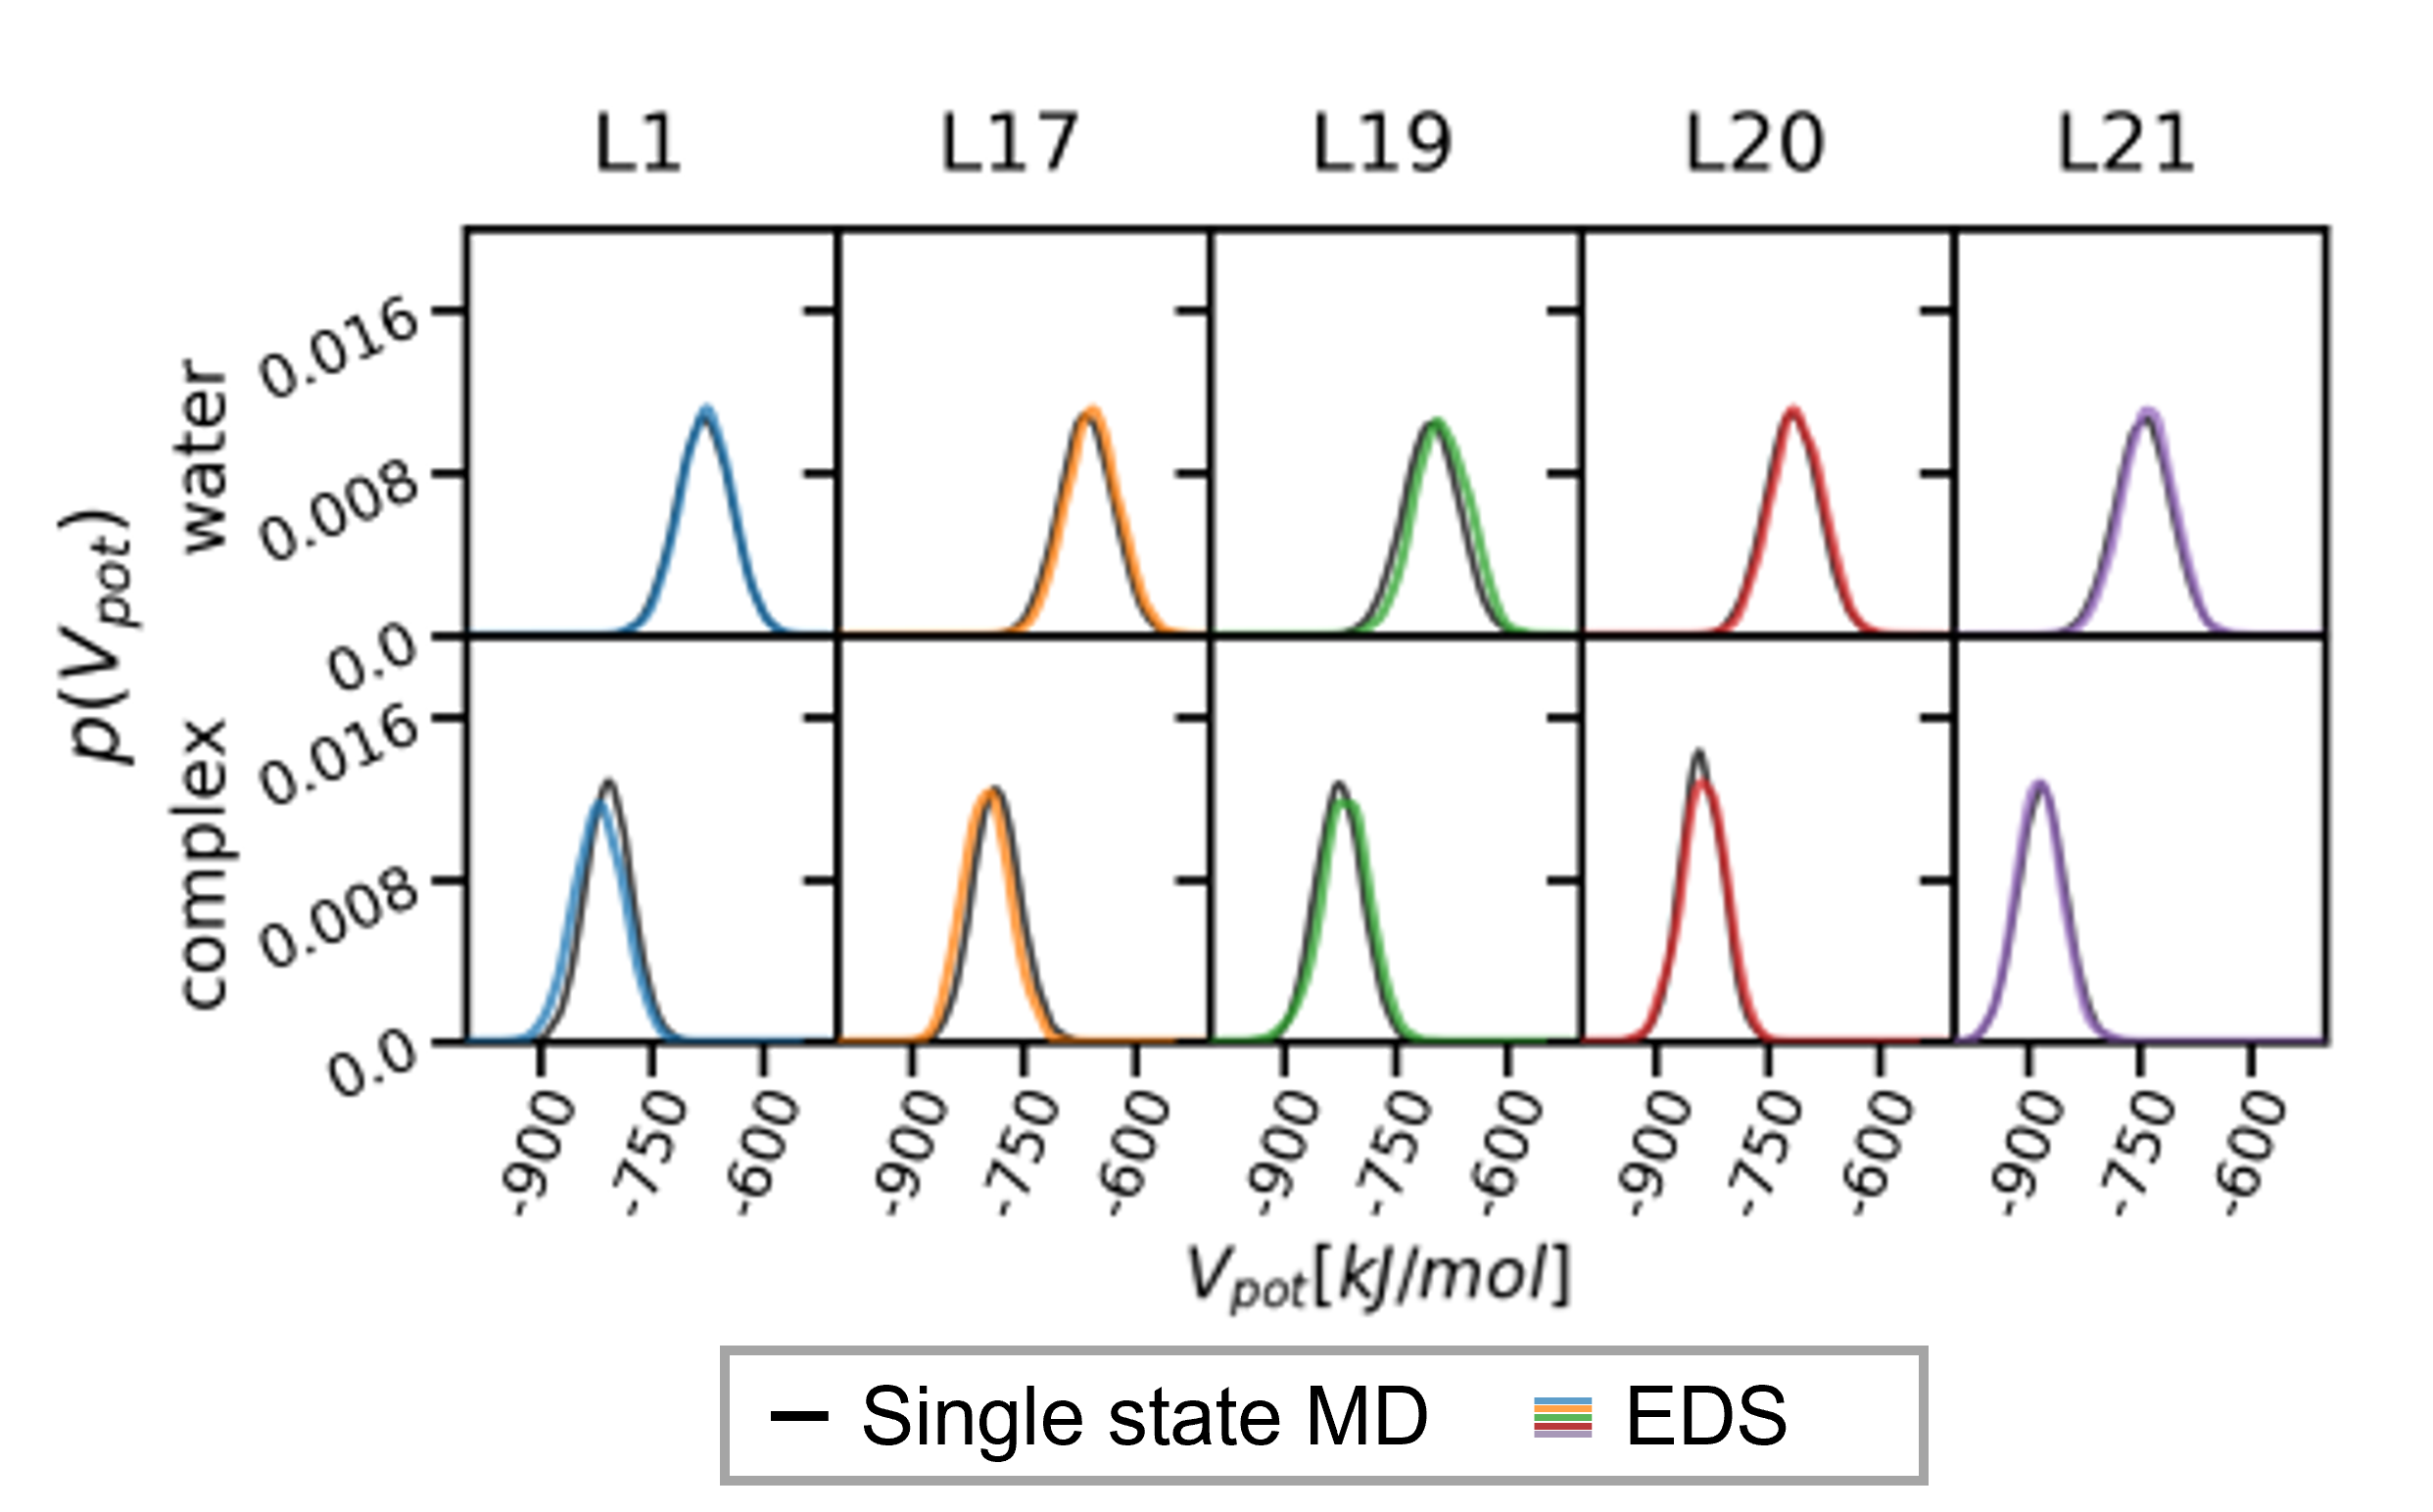
\includegraphics[width=0.8\textwidth]{fig/results/ringOpening/paramExploration/single_state_energy_sampling.png}
    \caption{Comparison of the potential-energy distribution obtained from a standard MD simulation of a given end state (black) and from an EDS simulation with the given end state favoured (colored) from the first step of the RE-EDS workflow.}
     \label{fig:CHK1_set2_stateOptimization_EnergyDistribution}
\end{figure}

\subsection{Energy Offset Estimation}
The relative energy offsets $\Delta \Delta E^R_{ji}$ are compared with the experimental relative binding free energies $\Delta \Delta G^\text{bind}_{ji}$ in Figure \ref{SIfig:Eoff_experiment_corr_RingOpening}. 
The RMSE between $\Delta \Delta E^R_{ji}$ obtained with RE-EDS 1SS and $\Delta \Delta G^\text{bind}_{ji}$ is $12.6$~kJ~mol$^{-1}$. Outliers are mainly related to L19.
With the RE-EDS SSM approach, the RMSE was reduced to $7.0$~kJ~mol$^{-1}$. No clear outliers were observed in this case. Thus, the use of the SSM approach is recommended for RE-EDS simulations.

%The energy offsets obtained with the SSM approach are shown as a function of the replica ($s$-value) in Figure \ref{SIfig:Eoff-perreplica}. 

\begin{figure}[H]
\centering
  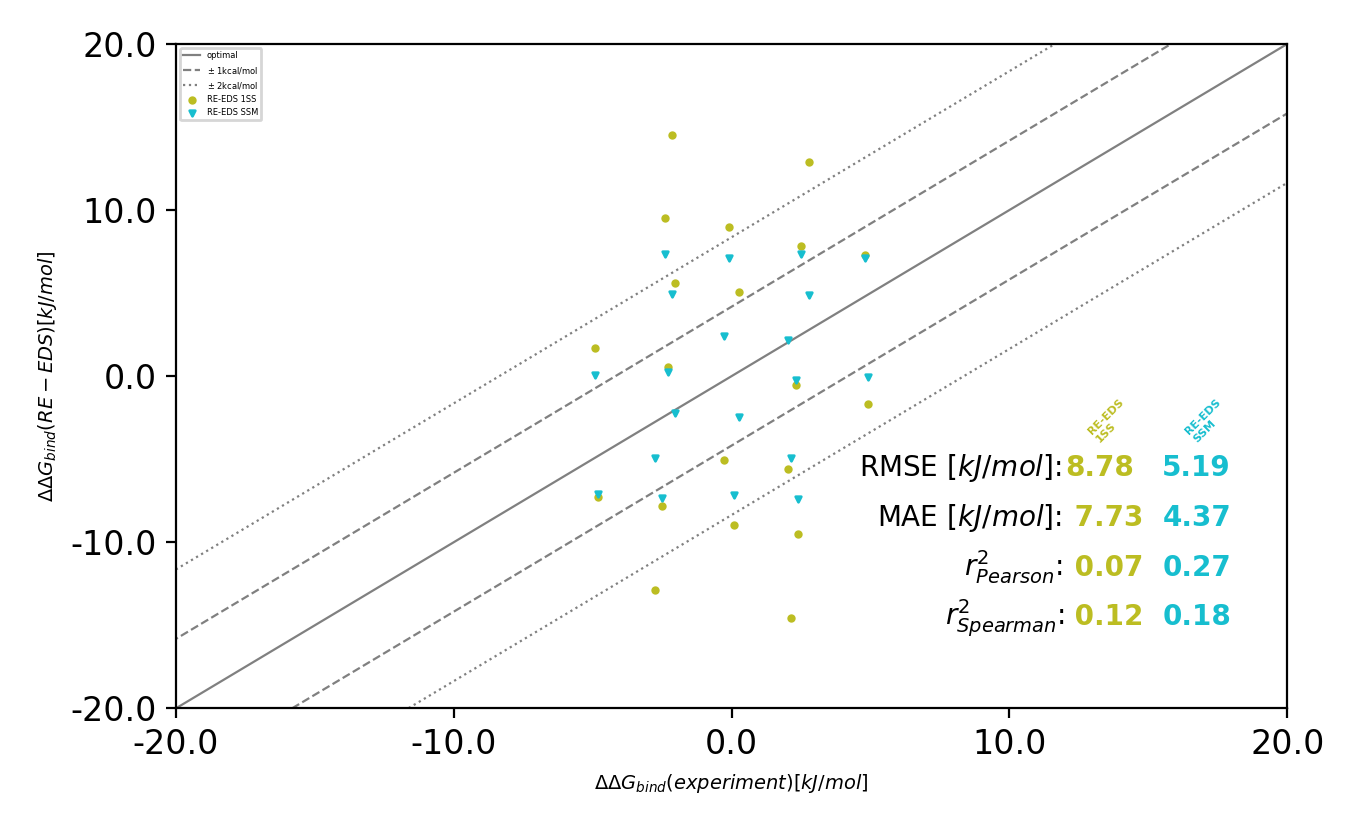
\includegraphics[width=0.8\textwidth]{fig/results/ringOpening/paramOptimization/RingClosure_system_Eoff_final_results.png}
\caption{Comparison of the relative energy offsets $\Delta \Delta E^R_{ji}$ in water and complex with the experimental relative binding free energies $\Delta \Delta G^\text{bind}_{ji}$. The energy offsets were estimated from RE-EDS simulations using the 1SS (green) or SSM (blue) approach to select the starting configurations of the replicas.} \label{SIfig:Eoff_experiment_corr_RingOpening}
\end{figure}


\subsection{Optimization of the $s$-Distribution and the energy offsets}
\begin{figure}[h]
\centering
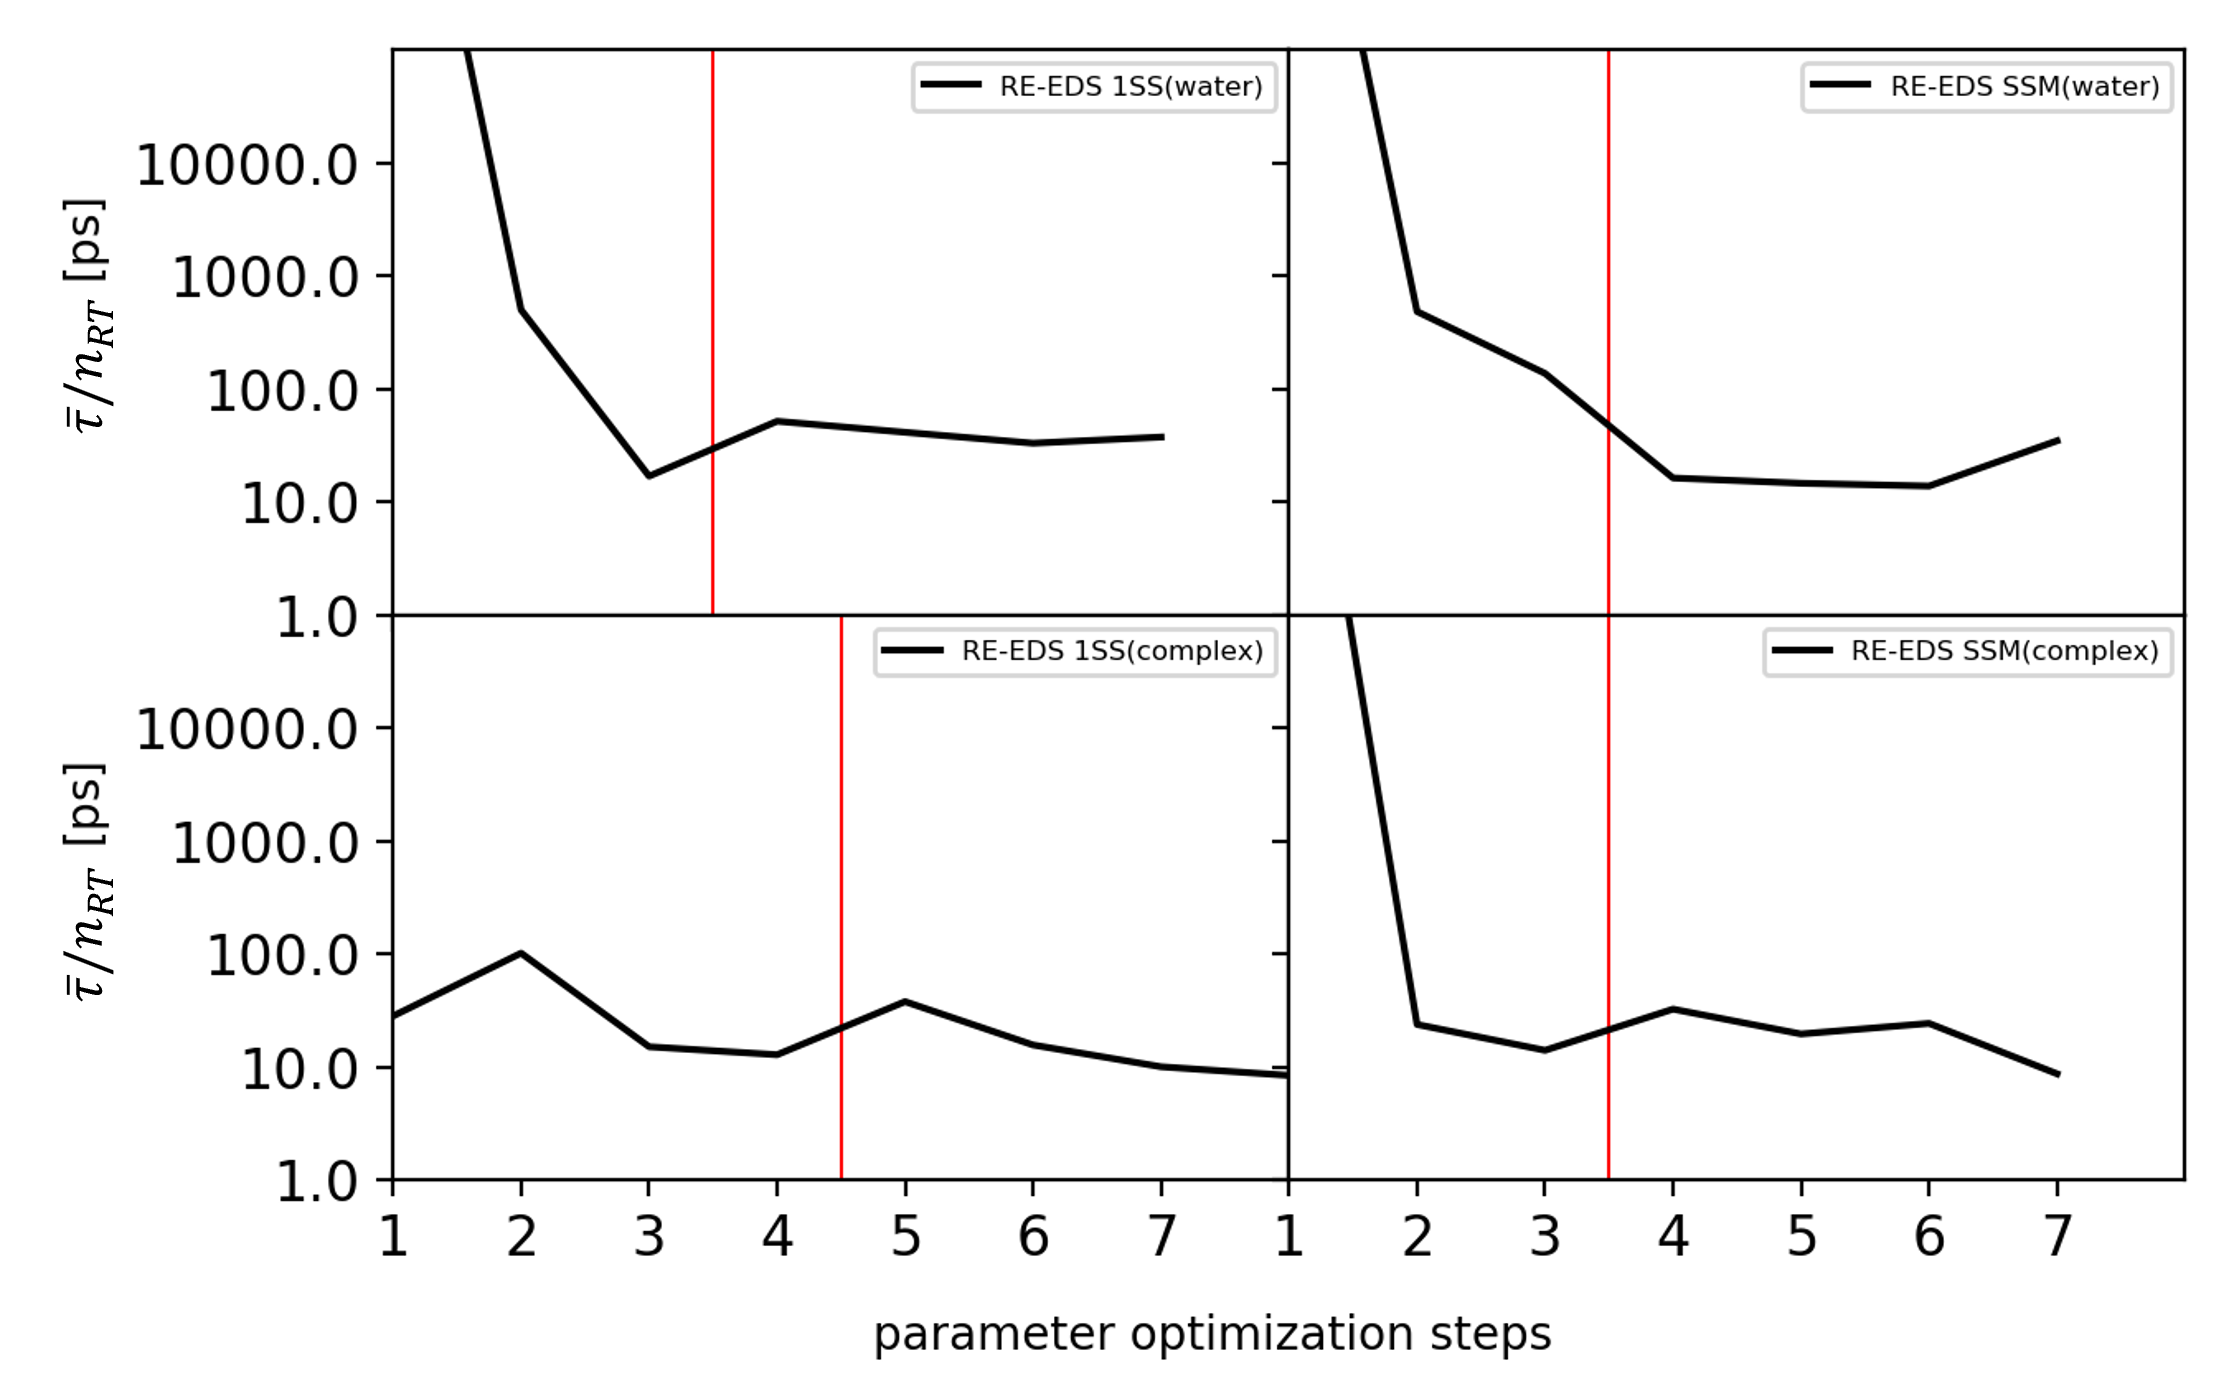
\includegraphics[width=\linewidth]{fig/results/ringOpening/paramOptimization/RingOpening_optimization_RTstat.png}
\caption{Average round-trip time as a function of the optimization steps $i$ ($\overline{\tau}_i$) on a logarithmic scale. The red line indicates the switch from $s$-optimization to energy offset rebalancing.}
\label{SIfig:CHK1_RingOpening_soptimization_efficiency}
\end{figure}

\begin{figure}[H]
\centering
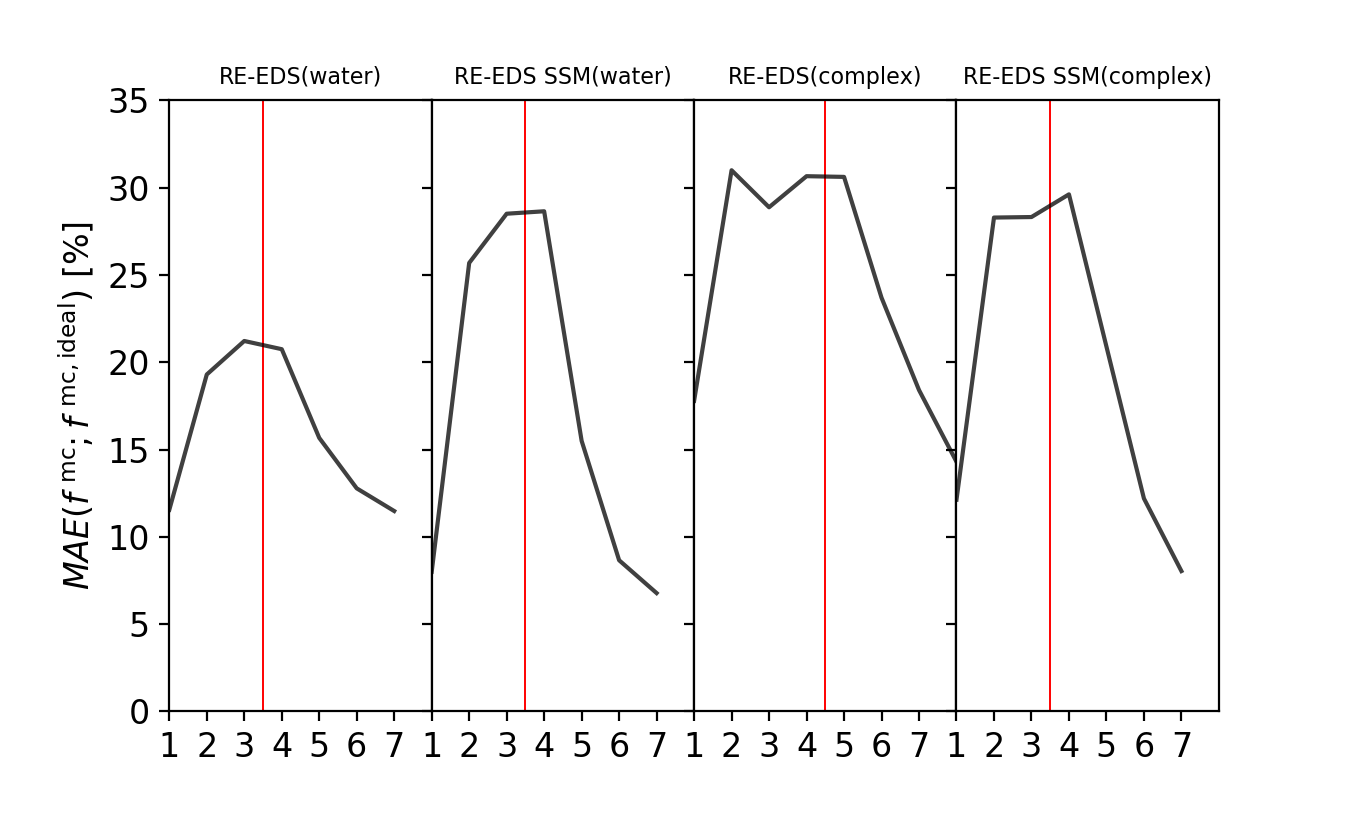
\includegraphics[width=\linewidth]{fig/results/ringOpening/paramOptimization/RingOpening_optimization_fractOptSampMAE.png}
\caption{Mean absolute deviation (MAE, in percentage) of the observed state sampling $f_i^{\text{mc}}$ from the ideal equal distribution $f_i^{\text{mc,ideal}}$ during the short optimization simulations. The red line indicates the switch from $s$-optimization to energy offset rebalancing.}
\label{SIfig:CHK1_RingOpening_optimization_fractOptSampMAE}
\end{figure}


\subsection{Free-Energy Calculation}
\begin{table}[H]
\caption{Free-energy differences in water and in complex calculated from the production run of 3.5~ns of length with the RE-EDS 1SS and RE-EDS SSM approaches.}
\begin{center}
\begin{tabular}{ c c |c c |c c}
  \multicolumn{2}{c|}{Ligand} & \multicolumn{2}{c|}{RE-EDS 1SS} &\multicolumn{2}{c}{RE-EDS SSM}\\ 
  J & I  & water [kJ~mol$^{-1}$] & complex [kJ~mol$^{-1}$]  & water [kJ~mol$^{-1}$] & complex [kJ~mol$^{-1}$] \\
  \hline
        L17 &         L1 &       11.9 $\pm$ 0.0&        17.0 $\pm$ 0.8&   12.4 $\pm$ 0.5&   9.4 $\pm$ 1.9\\
        L19 &         L1 &        2.7 $\pm$ 0.0&        5.7 $\pm$ 1.0&     3.1 $\pm$ 0.0&   8.0 $\pm$ 0.0\\
        L20 &         L1 &      -47.8 $\pm$ 0.0&      -47.6 $\pm$ 0.9& -47.7 $\pm$ 0.0&  -48.1 $\pm$ 0.0\\
        L21 &         L1 &      -61.7 $\pm$ 0.06&     -63.1 $\pm$ 0.8& -61.7 $\pm$ 0.0&  -64.8 $\pm$ 0.0\\
        L19 &         L17 &      -9.2 $\pm$ 0.0&      -11.3 $\pm$ 0.6&  -9.3 $\pm$ 0.5&   -1.4 $\pm$ 1.9\\
        L20 &         L17 &     -59.6 $\pm$ 0.0&      -64.5 $\pm$ 0.1& -60.1 $\pm$ 0.5&  -57.6 $\pm$ 1.9\\
        L21 &         L17 &     -73.6 $\pm$ 0.0&      -80.1 $\pm$ 0.1& -74.1 $\pm$ 0.5&  -74.3 $\pm$ 1.9\\
        L20 &         L19 &     -50.5 $\pm$ 0.0&      -53.2 $\pm$ 0.6& -50.7 $\pm$ 0.0&  -56.2 $\pm$ 0.0\\
        L21 &         L19 &     -64.4 $\pm$ 0.0&      -68.8 $\pm$ 0.6& -64.7 $\pm$ 0.0&  -72.9 $\pm$ 0.0\\
        L21 &         L20 &     -13.9 $\pm$ 0.0&      -15.5 $\pm$ 0.2& -14.0 $\pm$ 0.08& -16.7 $\pm$ 0.0 \\
\end{tabular}
\end{center}
\label{SItab: RE-EDS_FE_RingCycleOpening_dFs}
\end{table}

\begin{figure}[H]
\centering
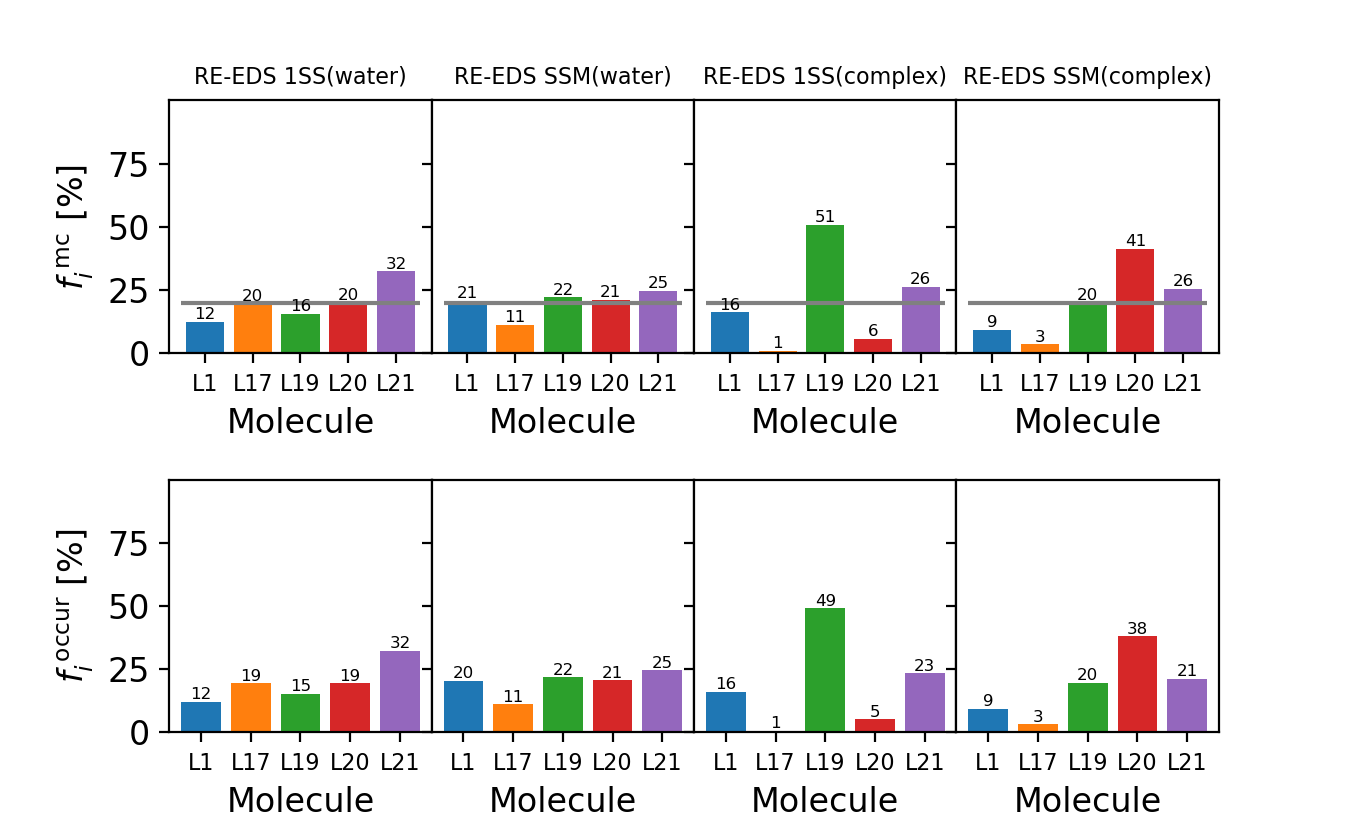
\includegraphics[width=\linewidth]{fig/results/ringOpening/FE/Reeds_RingOpening_production_sampling_s1.png}
\caption{Sampling of the end states in the final production run at replica $s=1.0$. Sampling was assessed by monitoring the maximally contributing end state (top panels) and by counting all end states a potential energy below $T_{i}^{phys}$ (see Table \ref{SItab:RingCycleOpenin_PotentialTresholds}) (bottom panels). Ideally, the sampling fraction as maximally contributing end state should be 1/$N$ (Eq. (8) in the main text) for all end states, indicated as a black horizontal line.}
\label{SIfig:CHK1_RingOpening_soptimization_final_Sampling_s1}
\end{figure}


\begin{figure}[H]
\centering
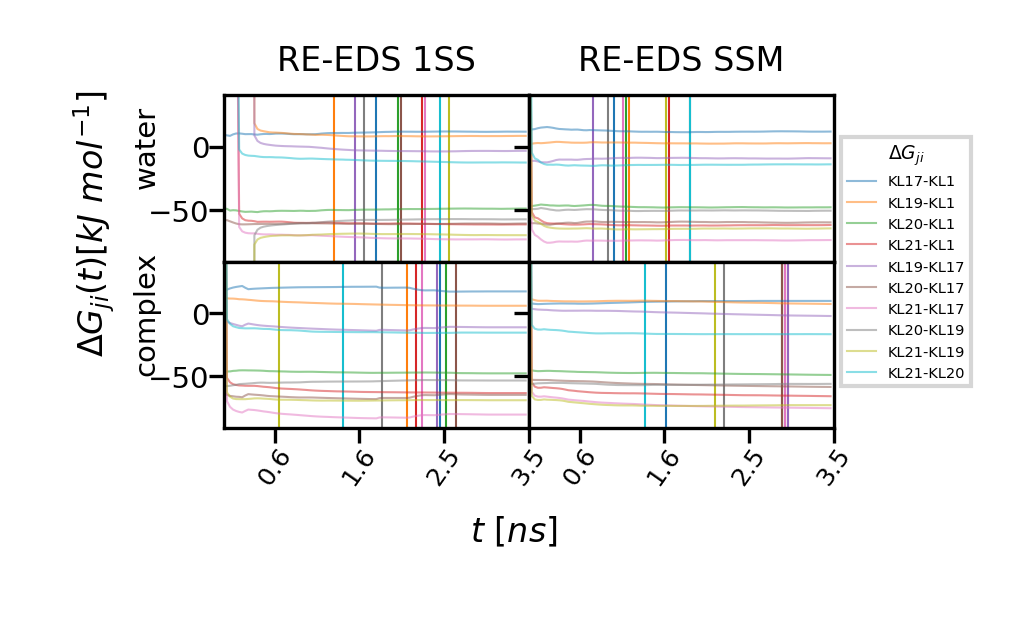
\includegraphics[width=\linewidth]{fig/results/ringOpening/FE/dF_RingOpening_Convergence.png}
\caption{Convergence analysis of the RE-EDS production runs (total 3.5~ns): The free-energy results are plotted as a function of the simulation time. The vertical lines indicate when a particular $\Delta G_{ji}$ value was found to be converged (deviation below 1~kJ~mol$^{-1}$).}
\label{SIfig:CHK1_RingOpening_dF_convergence}
\end{figure}


\clearpage
\newpage

%================================================================================
\section{Conclusion}
%================================================================================

This study reports the recent developments for the multistate free-energy method RE-EDS, which omits the definition of alchemical transition paths. The automatic workflow for RE-EDS was improved in robustness, and was applied to estimate the relative binding free energies of five CHK1 inhibitors containing typical core-hopping transformations. This system was investigated previously with FEP+ and QligFEP, allowing for a direct comparison of RE-EDS with state-of-the-art pairwise free-energy methods.
Using different starting configurations representing all end states (SSM approach) in the parameter optimization of the RE-EDS workflow improved the sampling, convergence, and the accuracy of the resulting free-energy differences. The performance of RE-EDS SSM was found to be comparable with FEP+ and QligFEP, and shows that RE-EDS with a ``dual topology" approach can be readily applied to challenging ligand transformations like ring size change, ring opening/closing, and ring extension.

In terms of computational efficiency, the total production run time with RE-EDS ($4$~ns per replica) was about half of that reported for FEP+ with this system. For RE-EDS, the simulation time could have been reduced further as the free-energy differences were found to be converged already after about $1$~ns. As multiple ligands are simulated simultaneously in a single RE-EDS simulation, this sampling enhancement will increase with increasing number of ligands. 
However, the pre-processing phase in the RE-EDS workflow currently uses a relatively large amount of simulation time. Making these steps more efficient will be addressed in future work.

The Python code for the RE-EDS workflow is provided on Github \\https://github.com/rinikerlab/reeds and can be used with the current version of GROMOS, freely available from http://www.gromos.net.

\clearpage
\pagebreak

%================================================================================
%\section{Appendix}
%================================================================================
\begin{ethappendix}
%================================================================================
%\appsection[CBTI and Quadrature]{quad}{Relationship between CBTI and Quadrature Integration}
%================================================================================

\end{ethappendix}
\clearpage
\pagebreak

%% %================================================================================
%% \begin{thebibliography}{74}
%% \input{\path/inc/paper.lrs}
%% \end{thebibliography}
%% %================================================================================

\end{document}
